\section{Experiments \& Results}
\subsection{Experimental Setup}
\label{sec:experimental_setup}
\textbf{Implementation \& Dataset Details:} 
We evaluate models across six standard benchmarks: 7-Scenes~\citep{7scenes1, 7scenes2}, NRGB-D~\citep{nrgdb_dataset}, and RotMV, presented in the main paper, and DTU~\citep{jensen2014largeDTU}, ETH3D~\citep{Schops_2019_CVPRETH3D1, schoeps2017cvprETH3D2}, Mip-NeRF 360~\citep{barron2022mipnerf360}, and Tanks \& Temples~\citep{Knapitsch2017tanksandtemples}, detailed in the supplementary (\cref{sec:additional_results_suppl}). Similarly, we include results for in-plane rotation (roll) in the main paper, with pitch and yaw results included in the supplementary \cref{sec:additional_results_suppl}

While our rendering-based rotation construction provides synthetically rotated sequences, it may not fully capture the characteristics of real-world rotated captures. 
Thus, we present a novel benchmark RotMV, consisting of seven real-world scenes (\textit{chairs}, \textit{foosball-table}, \textit{building}, \textit{rooftop}, \textit{room}, \textit{statue}, and \textit{table-tennis}). 
We capture each scene using a camera  in $4096\times3072$ resolution. 
Each scene is imaged from $16$ fixed viewpoints, and at each viewpoint, the camera is rolled in-plane through $12$ orientations spanning a full $360^\circ$ (in $30^\circ$ increments), resulting in $192$ images per scene.
For each viewpoint, we estimate the base camera pose from the upright ($0^\circ$) image using VGGT. 
The remaining $11$ roll-angle poses are derived analytically by applying the corresponding in-plane rotation to the base camera orientation, keeping the camera center and viewing direction fixed. Additional details about the dataset included visual examples is included in supplementary \cref{sec:rotmv_dataset}.
% We therefore introduce RotMV in \cref{sec:rotmv_dataset}, a curated benchmark of real paired upright and unconstrained rotated multi-view sequences, designed to facilitate evaluation of rotation robustness under authentic capture conditions. 
% Full dataset details and statistics are provided in the supplementary along with the results.
\\
\textbf{Evaluation Metrics:} 
Following the evaluation criteria of $\pi^3$ \citep{wang2025pi}, we use $16$-view input sequence and evaluate models on two tasks. For camera pose estimation, we report Rotation Accuracy ($\text{RAcc}_{30}$$\uparrow$), Translation Accuracy ($\text{TAcc}_{30}$$\uparrow$), and Area Under the Curve ($\text{AUC}_{30}$$\uparrow$) at a $30^\circ$ threshold \citep{wang2023posediffusion}, measuring the fraction of predictions within the threshold for rotation, translation, and both jointly. For point map estimation, we report Accuracy ($\text{Acc.}\downarrow$), Completeness ($\text{Comp.}\downarrow$), and Normal Consistency ($\text{N.C.}\uparrow$), the mean cosine similarity between predicted and ground-truth surface normals \citep{mast3r_eccv24}. 
\\
\textbf{Evaluation Protocol:} We vary the number of rotated views $m \in \{0, 4, 8, 12, 16\}$, corresponding to $\{0\%, 25\%, 50\%, 75\%, 100\%\}$ rotated view configurations. For each budget $m$, we select $m$ views uniformly at random and assign each an independent roll angles $\theta_i \sim \mathcal{U}(0^\circ, 360^\circ)$ (similarly for pitch and yaw), synthesizing rotated inputs via our controlled rotation synthesis. Ground-truth camera pose are updated to reflect the applied rotation angles and model predictions are aligned to ground truth using Umeyama \citep{umeyamaalgo}. We report the mean and standard deviation across $10$ independent random trials per $m$, unless noted otherwise. 

\vspace{-2mm}
\subsection{How Severe is Upright Bias?}
\label{sec:how_severe_is_upright_bias}

% \definecolor{datasetbg}{gray}{0.94}
% \begin{table*}[ht]
%     \centering
%     \caption{Point-map and camera-pose estimation performance under increasing fractions of rotated input views, measured by Normalized Consistency (N.C.) and $\mathrm{AUC}_{30}$, respectively. } 
%     \label{tab:rotation_degradation}
%     \small
%     %\renewcommand{\arraystretch}{1.2}
%     \setlength{\tabcolsep}{4.5pt}

%         \begin{tabular}{@{}ll ccccc ccccc@{}}
%         \toprule
%         & & \multicolumn{5}{c}{\textbf{Point-map Estimation (N.C.)}} & \multicolumn{5}{c}{\textbf{Camera Pose Estimation (AUC$_{30}$)}} \\
%         \cmidrule(lr){3-7} \cmidrule(lr){8-12}
%         & \textbf{Rot.}
%         & VGGT & VGGT-$\Omega$ & $\pi^3$ & MapAny. & DA3
%         & VGGT & VGGT-$\Omega$ & $\pi^3$ & MapAny. & DA3 \\
%         \midrule

%         % 7-Scenes (Unshaded)
%         & 0\%   & 82.4 & 80.7 & 78.9 & 81.3 & 79.6 & 91.2 & 89.8 & 88.4 & 90.1 & 89.2 \\
%         & 25\%  & 78.1 & 76.4 & 74.1 & 77.5 & 75.2 & 87.6 & 85.9 & 83.5 & 86.8 & 84.7 \\
%         & 50\%  & 71.5 & 69.8 & 68.2 & 72.1 & 69.5 & 82.3 & 80.7 & 78.1 & 82.5 & 79.3 \\
%         & 75\%  & 64.2 & 62.7 & 60.5 & 65.8 & 62.8 & 76.5 & 74.2 & 72.4 & 76.9 & 73.5 \\
%         \multirow{-5}{*}{\rotatebox[origin=c]{90}{\textbf{7-Scenes}}}
%         & 100\% & 57.8 & 55.3 & 53.7 & 59.2 & 55.6 & 69.4 & 67.8 & 65.9 & 70.3 & 66.7 \\
%         \addlinespace[3pt]

%         % NRGBD
%         \rowcolor{datasetbg}
%         & 0\%   & 84.1 & 82.6 & 80.2 & 83.5 & 81.4 & 92.4 & 91.3 & 90.2 & 92.0 & 91.0 \\
%         \rowcolor{datasetbg}
%         & 25\%  & 80.5 & 78.7 & 76.1 & 79.8 & 77.2 & 88.9 & 87.1 & 85.9 & 88.2 & 86.6 \\
%         \rowcolor{datasetbg}
%         & 50\%  & 75.2 & 73.4 & 70.8 & 74.6 & 72.1 & 84.1 & 82.8 & 81.0 & 83.7 & 81.9 \\
%         \rowcolor{datasetbg}
%         & 75\%  & 68.7 & 66.9 & 64.3 & 68.1 & 65.7 & 78.2 & 76.9 & 75.2 & 77.9 & 75.8 \\
%         \rowcolor{datasetbg}
%         \multirow{-5}{*}{\rotatebox[origin=c]{90}{\textbf{NRGBD}}}
%         & 100\% & 61.3 & 59.8 & 57.2 & 60.7 & 58.4 & 71.6 & 70.4 & 68.5 & 71.2 & 69.3 \\
%         \addlinespace[3pt]

%         % ETH3D
%         & 0\%   & 83.2 & 90.8 & 88.0 & 76.2 & 81.8 & 77.1 & 93.4 & 77.3 & 52.0 & 75.7 \\
%         & 25\%  & 78.5 & 86.4 & 84.5 & 74.6 & 81.6 & 67.1 & 93.1 & 75.1 & 50.5 & 76.8 \\
%         & 50\%  & 77.0 & 83.7 & 82.0 & 72.2 & 78.1 & 64.5 & 92.2 & 73.9 & 49.6 & 69.3 \\
%         & 75\%  & 72.9 & 81.8 & 79.3 & 70.9 & 77.4 & 59.8 & 89.9 & 68.8 & 47.7 & 69.8 \\
%         \multirow{-5}{*}{\rotatebox[origin=c]{90}{\textbf{ETH3D}}}
%         & 100\% & 66.2 & 77.1 & 74.4 & 64.0 & 72.3 & 54.8 & 84.9 & 62.7 & 39.5 & 60.6 \\
%         \bottomrule
%     \end{tabular}

% \end{table*}

%%%%%%%%%%%%%%%%%%%%%%%%%%%%%%%%%%%%%%%%%%%%%%%%%%%%%%%%%%%%%%%%%%%%%%%%%%%%%%%%%%%%%%%%%%%%%%%%%%%%%%%%%%%%%%


% \definecolor{datasetbg}{gray}{0.94}
% \begin{table*}[ht]
%     \centering
%     \caption{Point-map and camera-pose estimation performance under increasing fractions of rotated input views, measured by Normalized Consistency (N.C.) and $\mathrm{AUC}_{30}$, respectively. \sirjanh{This table's data doesnt match with generated result, need to confirm with Anudeep and correct it with the  } } 
%     \label{tab:rotation_degradation}
%     \small
%     %\renewcommand{\arraystretch}{1.2}
%     \setlength{\tabcolsep}{4.5pt}

%         \begin{tabular}{@{}ll ccccc ccccc@{}}
%         \toprule
%         & & \multicolumn{5}{c}{\textbf{Point-map Estimation (N.C.)}} & \multicolumn{5}{c}{\textbf{Camera Pose Estimation (AUC$_{30}$)}} \\
%         \cmidrule(lr){3-7} \cmidrule(lr){8-12}
%         & \textbf{Rot.}
%         & VGGT & VGGT-$\Omega$ & $\pi^3$ & MapAny. & DA3
%         & VGGT & VGGT-$\Omega$ & $\pi^3$ & MapAny. & DA3 \\
%         \midrule

%         % 7-Scenes (Unshaded)
%         & 0\%   & 0.824 & 0.807 & 0.789 & 0.813 & 0.796 & 91.2 & 89.8 & 88.4 & 90.1 & 89.2 \\
%         & 25\%  & 0.781 & 0.764 & 0.741 & 0.775 & 0.752 & 87.6 & 85.9 & 83.5 & 86.8 & 84.7 \\
%         & 50\%  & 0.715 & 0.698 & 0.682 & 0.721 & 0.695 & 82.3 & 80.7 & 78.1 & 82.5 & 79.3 \\
%         & 75\%  & 0.642 & 0.627 & 0.605 & 0.658 & 0.628 & 76.5 & 74.2 & 72.4 & 76.9 & 73.5 \\
%         \multirow{-5}{*}{\rotatebox[origin=c]{90}{\textbf{7-Scenes}}}
%         & 100\% & 0.578 & 0.553 & 0.537 & 0.592 & 0.556 & 69.4 & 67.8 & 65.9 & 70.3 & 66.7 \\
%         \addlinespace[3pt]

%         % NRGBD
%         \rowcolor{datasetbg}
%         & 0\%   & 0.841 & 0.826 & 0.802 & 0.835 & 0.814 & 92.4 & 91.3 & 90.2 & 92.0 & 91.0 \\
%         \rowcolor{datasetbg}
%         & 25\%  & 0.805 & 0.787 & 0.761 & 0.798 & 0.772 & 88.9 & 87.1 & 85.9 & 88.2 & 86.6 \\
%         \rowcolor{datasetbg}
%         & 50\%  & 0.752 & 0.734 & 0.708 & 0.746 & 0.721 & 84.1 & 82.8 & 81.0 & 83.7 & 81.9 \\
%         \rowcolor{datasetbg}
%         & 75\%  & 0.687 & 0.669 & 0.643 & 0.681 & 0.657 & 78.2 & 76.9 & 75.2 & 77.9 & 75.8 \\
%         \rowcolor{datasetbg}
%         \multirow{-5}{*}{\rotatebox[origin=c]{90}{\textbf{NRGBD}}}
%         & 100\% & 0.613 & 0.598 & 0.572 & 0.607 & 0.584 & 71.6 & 70.4 & 68.5 & 71.2 & 69.3 \\
%         \addlinespace[3pt]

%         % ETH3D
%         & 0\%   & 0.832 & 0.908 & 0.880 & 0.762 & 0.818 & 77.1 & 93.4 & 77.3 & 52.0 & 75.7 \\
%         & 25\%  & 0.785 & 0.864 & 0.845 & 0.746 & 0.816 & 67.1 & 93.1 & 75.1 & 50.5 & 76.8 \\
%         & 50\%  & 0.770 & 0.837 & 0.820 & 0.722 & 0.781 & 64.5 & 92.2 & 73.9 & 49.6 & 69.3 \\
%         & 75\%  & 0.729 & 0.818 & 0.793 & 0.709 & 0.774 & 59.8 & 89.9 & 68.8 & 47.7 & 69.8 \\
%         \multirow{-5}{*}{\rotatebox[origin=c]{90}{\textbf{ETH3D}}}
%         & 100\% & 0.662 & 0.771 & 0.744 & 0.640 & 0.723 & 54.8 & 84.9 & 62.7 & 39.5 & 60.6 \\
%         \bottomrule
%     \end{tabular}

% \end{table*}


%%%%%%%%%%%%%%%%%%%%%%%%%%%%%%%%%%%%%%%%%%%%%%%%%%%%%%%%%%%%%%%%%%%%%%%%%%%%%%%%%%%%%%%%%%%%%%%%%%%%%%%%%%%%%%
% Final Version. 

% \definecolor{datasetbg}{gray}{0.94}
% \begin{table*}[ht]
%     \centering
%     \caption{Point-map and camera-pose estimation performance under increasing fractions of rotated input views, measured by Normalized Consistency (N.C.) and $\mathrm{AUC}_{30}$, respectively.}
%     \label{tab:rotation_degradation}
%     \small
%     \setlength{\tabcolsep}{4.5pt}

%     \begin{tabular}{@{}ll ccccc ccccc@{}}
%         \toprule
%         & & \multicolumn{5}{c}{\textbf{Point-map Estimation (N.C.)}}
%         & \multicolumn{5}{c}{\textbf{Camera Pose Estimation (AUC$_{30}$)}} \\
%         \cmidrule(lr){3-7} \cmidrule(lr){8-12}
%         & \textbf{Rot.}
%         & VGGT & VGGT-$\Omega$ & $\pi^3$ & MapA. & DA3
%         & VGGT & VGGT-$\Omega$ & $\pi^3$ & MapA. & DA3 \\
%         \midrule

%         % 7-Scenes
%         & 0\%   & 0.658 $\pm$ 0.034 & 0.666 $\pm$ 0.046 & 0.673 $\pm$ 0.047 & 0.628 $\pm$ 0.050 & 0.673 $\pm$ 0.036 & 86.6 $\pm$ 6.6 & 87.5 $\pm$ 9.0 & 87.5 $\pm$ 6.0 & 80.9 $\pm$ 15.4 & 88.2 $\pm$ 7.2 \\
%         & 25\%   & 0.632 $\pm$ 0.030 & 0.666 $\pm$ 0.005 & 0.641 $\pm$ 0.022 & 0.606 $\pm$ 0.020 & 0.648 $\pm$ 0.025 & 70.0 $\pm$ 13.2 & 84.1 $\pm$ 2.5 & 71.6 $\pm$ 6.8 & 53.7 $\pm$ 10.9 & 71.2 $\pm$ 11.0 \\
%         &50\%   & 0.616 $\pm$ 0.038 & 0.669 $\pm$ 0.008 & 0.626 $\pm$ 0.029 & 0.595 $\pm$ 0.027 & 0.635 $\pm$ 0.032 & 54.6 $\pm$ 19.2 & 81.1 $\pm$ 4.1 & 59.0 $\pm$ 10.3 & 37.0 $\pm$ 11.3 & 55.4 $\pm$ 16.4 \\
%         & 75\%   & 0.601 $\pm$ 0.040 & 0.671 $\pm$ 0.007 & 0.619 $\pm$ 0.030 & 0.588 $\pm$ 0.022 & 0.624 $\pm$ 0.029 & 44.3 $\pm$ 18.8 & 76.0 $\pm$ 6.6 & 49.4 $\pm$ 10.3 & 27.4 $\pm$ 9.5 & 51.8 $\pm$ 11.2 \\
%         \multirow{-5}{*}{\rotatebox[origin=c]{90}{\textbf{7-Scenes}}}
%         & 100\% & 0.604 $\pm$ 0.030 & 0.662 $\pm$ 0.015 & 0.609 $\pm$ 0.028 & 0.584 $\pm$ 0.024 & 0.633 $\pm$ 0.019 & 43.8 $\pm$ 10.4 & 70.4 $\pm$ 6.6 & 45.3 $\pm$ 8.7 & 23.7 $\pm$ 6.6 & 53.3 $\pm$ 9.9 \\
%         \addlinespace[3pt]

%         % NRGBD
%         \rowcolor{datasetbg}
%         & 0\%   & 0.802 $\pm$ 0.032 & 0.830 $\pm$ 0.038 & 0.809 $\pm$ 0.063 & 0.749 $\pm$ 0.052 & 0.822 $\pm$ 0.035 & 98.6 $\pm$ 1.2 & 99.3 $\pm$ 0.6 & 96.4 $\pm$ 1.9 & 93.9 $\pm$ 4.3 & 99.9 $\pm$ 0.2 \\
%         \rowcolor{datasetbg}
%         & 25\%   & 0.742 $\pm$ 0.044 & 0.810 $\pm$ 0.016 & 0.757 $\pm$ 0.037 & 0.706 $\pm$ 0.033 & 0.749 $\pm$ 0.056 & 88.5 $\pm$ 9.6 & 96.6 $\pm$ 2.0 & 86.8 $\pm$ 7.2 & 69.0 $\pm$ 14.2 & 83.5 $\pm$ 13.1 \\
%         \rowcolor{datasetbg}
%         & 50\%   & 0.721 $\pm$ 0.046 & 0.792 $\pm$ 0.014 & 0.732 $\pm$ 0.035 & 0.667 $\pm$ 0.049 & 0.721 $\pm$ 0.071 & 78.5 $\pm$ 14.4 & 94.2 $\pm$ 2.3 & 78.4 $\pm$ 8.3 & 49.1 $\pm$ 14.6 & 72.4 $\pm$ 16.1 \\
%         \rowcolor{datasetbg}
%         & 75\%   & 0.705 $\pm$ 0.054 & 0.773 $\pm$ 0.011 & 0.722 $\pm$ 0.036 & 0.649 $\pm$ 0.046 & 0.706 $\pm$ 0.071 & 73.4 $\pm$ 15.6 & 91.4 $\pm$ 3.1 & 75.9 $\pm$ 10.0 & 37.0 $\pm$ 14.7 & 65.0 $\pm$ 17.1 \\
%         \rowcolor{datasetbg}
%         \multirow{-5}{*}{\rotatebox[origin=c]{90}{\textbf{NRGBD}}}
%         & 100\% & 0.709 $\pm$ 0.058 & 0.763 $\pm$ 0.007 & 0.717 $\pm$ 0.038 & 0.629 $\pm$ 0.042 & 0.716 $\pm$ 0.059 & 70.4 $\pm$ 16.1 & 89.3 $\pm$ 2.7 & 73.5 $\pm$ 9.0 & 27.3 $\pm$ 11.7 & 69.9 $\pm$ 17.8 \\
%         \addlinespace[3pt]

%     \end{tabular}

% \end{table*}

\definecolor{datasetbg}{gray}{0.94}
% Helper command to shift std dev right using left-alignment and offset spacing
\newcommand{\valstd}[2]{\shortstack[l]{#1 \\ {\tiny\hspace*{0.4em}$\pm$#2}}}

\begin{table*}[t]
    \centering
    \caption{\textbf{Point-map and camera-pose estimation.} Performance under increasing fractions of rotated input views measured by Normal Consistency (N.C.) and $\mathrm{AUC}_{30}$, respectively.}
    \label{tab:rotation_degradation_main}
    \small
    \setlength{\tabcolsep}{4.5pt}

    \begin{tabular}{@{}ll ccccc ccccc@{}}
        \toprule
        & & \multicolumn{5}{c}{\textbf{Point-map Estimation (N.C.)}}
        & \multicolumn{5}{c}{\textbf{Camera Pose Estimation (AUC$_{30}$)}} \\
        \cmidrule(lr){3-7} \cmidrule(lr){8-12}
        & \textbf{Rot.}
        & VGGT & VGGT-$\Omega$ & $\pi^3$ & MapA. & DA3
        & VGGT & VGGT-$\Omega$ & $\pi^3$ & MapA. & DA3 \\
        \midrule

        % 7-Scenes
        & 0\%   & \valstd{0.658}{0.034} & \valstd{0.666}{0.046} & \valstd{0.673}{0.047} & \valstd{0.628}{0.050} & \valstd{0.673}{0.036} & \valstd{86.6}{6.6} & \valstd{87.5}{9.0} & \valstd{87.5}{6.0} & \valstd{80.9}{15.4} & \valstd{88.2}{7.2} \\
        & 25\%  & \valstd{0.632}{0.030} & \valstd{0.666}{0.005} & \valstd{0.641}{0.022} & \valstd{0.606}{0.020} & \valstd{0.648}{0.025} & \valstd{70.0}{13.2} & \valstd{84.1}{2.5} & \valstd{71.6}{6.8} & \valstd{53.7}{10.9} & \valstd{71.2}{11.0} \\
        & 50\%  & \valstd{0.616}{0.038} & \valstd{0.669}{0.008} & \valstd{0.626}{0.029} & \valstd{0.595}{0.027} & \valstd{0.635}{0.032} & \valstd{54.6}{19.2} & \valstd{81.1}{4.1} & \valstd{59.0}{10.3} & \valstd{37.0}{11.3} & \valstd{55.4}{16.4} \\
        & 75\%  & \valstd{0.601}{0.040} & \valstd{0.671}{0.007} & \valstd{0.619}{0.030} & \valstd{0.588}{0.022} & \valstd{0.624}{0.029} & \valstd{44.3}{18.8} & \valstd{76.0}{6.6} & \valstd{49.4}{10.3} & \valstd{27.4}{9.5} & \valstd{51.8}{11.2} \\
        \multirow{-7}{*}{\rotatebox[origin=c]{90}{\textbf{7-Scenes}}}
        & 100\% & \valstd{0.604}{0.030} & \valstd{0.662}{0.015} & \valstd{0.609}{0.028} & \valstd{0.584}{0.024} & \valstd{0.633}{0.019} & \valstd{43.8}{10.4} & \valstd{70.4}{6.6} & \valstd{45.3}{8.7} & \valstd{23.7}{6.6} & \valstd{53.3}{9.9} \\
        \addlinespace[3pt]

        % NRGBD
        \rowcolor{datasetbg}
        & 0\%   & \valstd{0.802}{0.032} & \valstd{0.830}{0.038} & \valstd{0.809}{0.063} & \valstd{0.749}{0.052} & \valstd{0.822}{0.035} & \valstd{98.6}{1.2} & \valstd{99.3}{0.6} & \valstd{96.4}{1.9} & \valstd{93.9}{4.3} & \valstd{99.9}{0.2} \\
        \rowcolor{datasetbg}
        & 25\%  & \valstd{0.742}{0.044} & \valstd{0.810}{0.016} & \valstd{0.757}{0.037} & \valstd{0.706}{0.033} & \valstd{0.749}{0.056} & \valstd{88.5}{9.6} & \valstd{96.6}{2.0} & \valstd{86.8}{7.2} & \valstd{69.0}{14.2} & \valstd{83.5}{13.1} \\
        \rowcolor{datasetbg}
        & 50\%  & \valstd{0.721}{0.046} & \valstd{0.792}{0.014} & \valstd{0.732}{0.035} & \valstd{0.667}{0.049} & \valstd{0.721}{0.071} & \valstd{78.5}{14.4} & \valstd{94.2}{2.3} & \valstd{78.4}{8.3} & \valstd{49.1}{14.6} & \valstd{72.4}{16.1} \\
        \rowcolor{datasetbg}
        & 75\%  & \valstd{0.705}{0.054} & \valstd{0.773}{0.011} & \valstd{0.722}{0.036} & \valstd{0.649}{0.046} & \valstd{0.706}{0.071} & \valstd{73.4}{15.6} & \valstd{91.4}{3.1} & \valstd{75.9}{10.0} & \valstd{37.0}{14.7} & \valstd{65.0}{17.1} \\
        \rowcolor{datasetbg}
        \multirow{-7}{*}{\rotatebox[origin=c]{90}{\textbf{NRGB-D}}}
        & 100\% & \valstd{0.709}{0.058} & \valstd{0.763}{0.007} & \valstd{0.717}{0.038} & \valstd{0.629}{0.042} & \valstd{0.716}{0.059} & \valstd{70.4}{16.1} & \valstd{89.3}{2.7} & \valstd{73.5}{9.0} & \valstd{27.3}{11.7} & \valstd{69.9}{17.8} \\
        \addlinespace[3pt]

        % ETH3D
        & 0\%   & \valstd{0.832}{0.074} & \valstd{0.908}{0.038} & \valstd{0.880}{0.049} & \valstd{0.762}{0.141} & \valstd{0.818}{0.129} & \valstd{77.1}{17.2} & \valstd{93.4}{5.3} & \valstd{77.3}{15.2} & \valstd{52.0}{26.7} & \valstd{75.7}{26.2} \\
        & 25\%  & \valstd{0.785}{0.096} & \valstd{0.864}{0.079} & \valstd{0.845}{0.083} & \valstd{0.746}{0.126} & \valstd{0.816}{0.111} & \valstd{67.1}{25.4} & \valstd{93.1}{5.6} & \valstd{75.1}{17.1} & \valstd{50.5}{24.1} & \valstd{76.8}{23.5} \\
        & 50\%  & \valstd{0.770}{0.089} & \valstd{0.837}{0.085} & \valstd{0.820}{0.090} & \valstd{0.722}{0.123} & \valstd{0.781}{0.122} & \valstd{64.5}{24.2} & \valstd{92.2}{6.4} & \valstd{73.9}{17.5} & \valstd{49.6}{24.2} & \valstd{69.3}{27.6} \\
        & 75\%  & \valstd{0.729}{0.103} & \valstd{0.818}{0.097} & \valstd{0.793}{0.101} & \valstd{0.709}{0.126} & \valstd{0.774}{0.126} & \valstd{59.8}{27.5} & \valstd{89.9}{8.3} & \valstd{68.8}{22.4} & \valstd{47.7}{23.4} & \valstd{69.8}{29.2} \\
        \multirow{-7}{*}{\rotatebox[origin=c]{90}{\textbf{ETH3D}}}
        & 100\% & \valstd{0.662}{0.130} & \valstd{0.771}{0.097} & \valstd{0.744}{0.101} & \valstd{0.640}{0.124} & \valstd{0.723}{0.117} & \valstd{54.8}{29.4} & \valstd{84.9}{10.4} & \valstd{62.7}{23.1} & \valstd{39.5}{26.2} & \valstd{60.6}{31.4} \\
        \bottomrule

    \end{tabular}
\vspace{-3mm}
\end{table*}

To evaluate whether arbitrary image rotations constitute a meaningful failure mode for feed-forward 3D reconstruction models, we measure performance across the rotation budgets. ~\Cref{tab:rotation_degradation_main} reveals consistent and severe degradation across all models and datasets as the fraction of rotated views increases. On 7-Scenes, camera pose estimation ($\mathrm{AUC}_{30}$) drops for all models, with absolute declines ranging from $17.1$ points (VGGT-$\Omega$: $87.5$ to $70.4$) to $57.2$ points (MapA.: $80.9$ to $23.7$) at $100\%$ rotation. Point-map quality (N.C.) follows the same trend across all models. On NRGB-D, degradation is similarly consistent and universal, with pose accuracy falling by $10.2-66.6$ points depending on the model. On ETH3D, all models exhibit substantial declines in both metrics, with $\mathrm{AUC}_{30}$ dropping by $8.5$--$22.3$ points at full rotation. Across all three datasets, these results confirm that UprightBias is a systematic and severe failure mode affecting all evaluated feed-forward reconstruction models. Results on the remaining dataset along with pitch and yaw are included in supplementary \cref{sec:additional_results_suppl}.


% \textcolor{blue}{ Across all three datasets and evaluated models, both point-map and camera-pose estimation consistently deteriorate as the fraction of rotated input views increases, with the largest drops observed when $100\%$ views are rotated.
% On 7-Scenes and NRGB-D, the degradation is largely monotonic across all models, with MapA. retaining the strongest performance at higher rotation fractions and $\pi^3$ generally exhibiting the largest drop.
% On ETH3D, the models show substantially different sensitivities: VGGT-$\Omega$ remains comparatively robust to rotation, with N.C. decreasing from 0.908 to 0.771 and $\mathrm{AUC}_{30}$ from 93.4 to 84.9, while MapA. exhibits a larger relative decline, particularly in camera pose estimation (52.0 to 39.5).
% VGGT similarly shows a pronounced reduction in pose accuracy on ETH3D, with $\mathrm{AUC}_{30}$ falling from 77.1 to 54.8 as all views become rotated.}



\subsection{What Causes this Upright Bias?}
\label{ssec:data_audit}
% Having established that arbitrary image rotations consistently degrade reconstruction quality, we next investigate the origin of this behavior. 
% We hypothesize that it reflects a statistical property shared by the training data used by current feed-forward reconstruction models.
% To evaluate this hypothesis, we perform a comprehensive data audit across the training corpora of state-of-the-art feed-forward geometric models, including VGGT, VGGT-$\Omega$, DA3, MapA, and $\pi^3$.
% As summarized in Table~\ref{tab:summary_training_data}, our audit reveals a striking trend, the overwhelming majority of training datasets used across all models are gravity-aligned by construction. \Badri{What is the meaning of gravity aligned is also needed. Also mention that detail audit is in supplementary}


\vspace{-2mm}
\begin{wraptable}{r}{0.4\textwidth}
    \vspace{-1mm}
    \centering
    \setlength{\tabcolsep}{2pt}
    \caption{\textbf{Dataset Audit. } Majority of training data across all models is Upright by construction}
    \label{tab:summary_training_data}
    \small
    \resizebox{\linewidth}{!}{
    \begin{tabular}{@{}llccccc@{}}
    \toprule
    \multicolumn{2}{l}{\textbf{Dataset}}               & \textbf{VGGT} & \textbf{VGGT-$\Omega$} & \textbf{DA3} & \textbf{MapA} & \textbf{$\pi^3$} \\ \midrule
    \multicolumn{2}{l}{\textbf{Fully Upright}} & \textbf{13}   & \textbf{18}            & \textbf{19}  & \textbf{10}   & \textbf{11}      \\
    \multicolumn{2}{l}{\textbf{Partially Upright}}     & \textbf{1}    & \textbf{2}             & \textbf{1}   & \textbf{0}    & \textbf{2}       \\ \bottomrule
    \end{tabular}
    }
    % \vspace{-1mm}
\end{wraptable}
Having established that rotations consistently degrade reconstruction quality, we investigate the origin of this behavior. 
% We define a dataset as \textbf{gravity-aligned} if its images are captured with the camera's vertical axis parallel to gravity as in handheld scans, street-level cameras etc leaving arbitrary in-plane rolls absent from the training distribution. 
As summarized in Table~\ref{tab:summary_training_data}, a comprehensive audit of the training corpora of VGGT, VGGT-$\Omega$, DA3, MapA., and $\pi^3$ reveals that the overwhelming majority of training datasets are upright by construction, spanning indoor RGB-D benchmarks, outdoor photo collections, and synthetic datasets alike. Consequently, feed-forward models learn a strong implicit prior that the camera and world coordinate systems share an aligned gravity vector, which fails when rotated inputs are encountered at inference time. A detailed dataset-by-dataset breakdown is provided in the supplementary \cref{sec:training_data_rebalancing}.

\subsection{Can ROVER Mitigate Upright Bias?} 
Having established the existence and origin of UprightBias, we investigate whether its effects can be mitigated entirely at inference time specifically, whether canonicalizing input orientations before reconstruction is sufficient to recover performance without any architectural modification or retraining. We compare each model in two settings: \emph{Baseline}, where rotated inputs are provided directly to the original model, and \emph{Ours}, where inputs are first canonicalized using ROVER and then passed to the unchanged model. Both settings are averaged over the same rotation-fraction sweep used in \cref{sec:how_severe_is_upright_bias}. Analogous experiments with are included in the supplementary.
\begin{figure*}
    \centering
    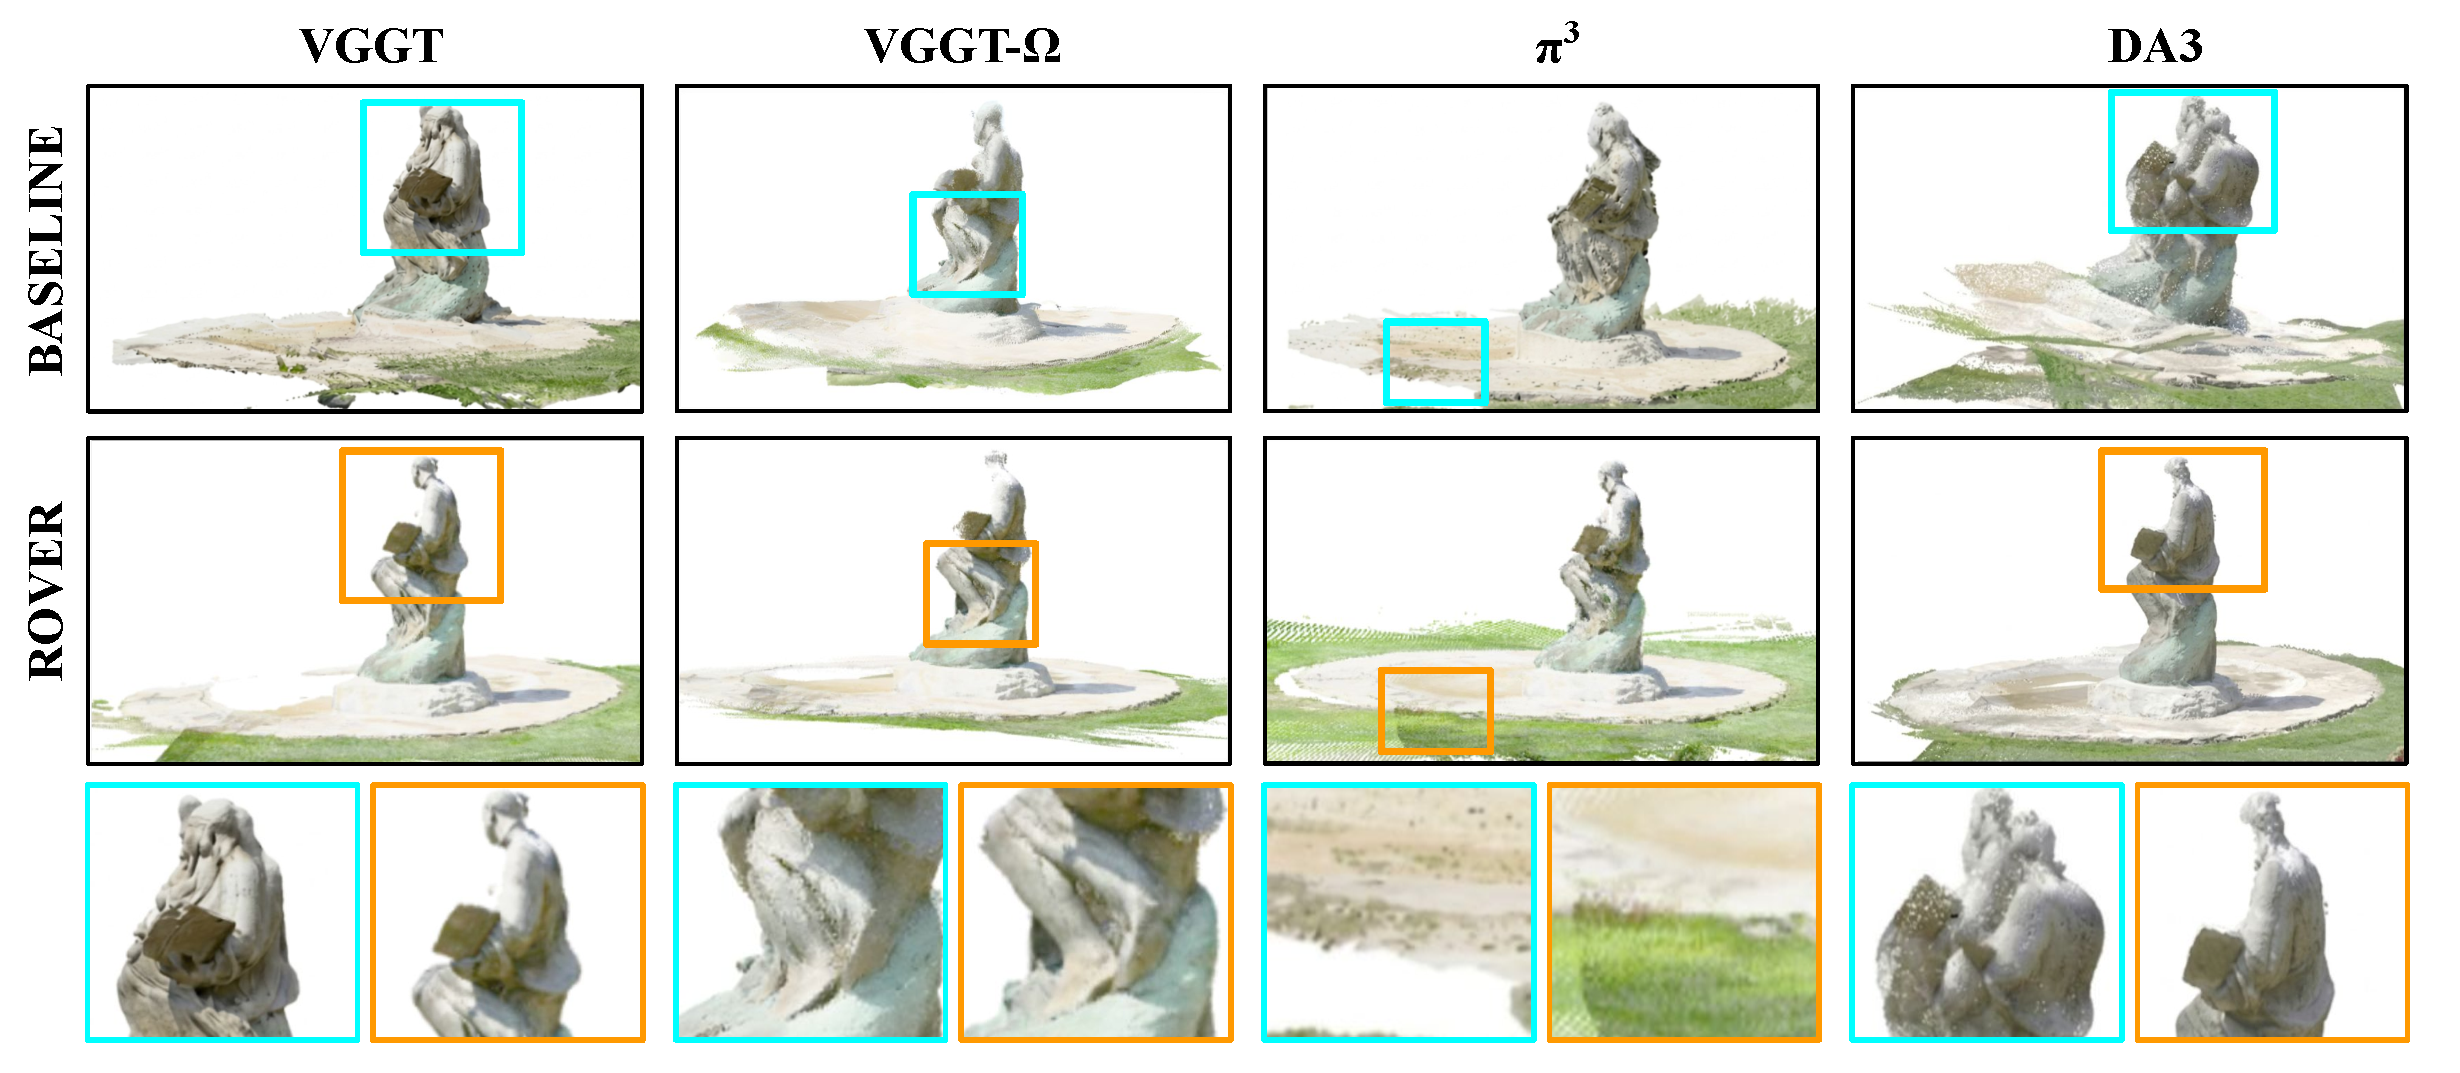
\includegraphics[width=\linewidth]{Figures/fig4/fig4.pdf}
    \caption{\textbf{Qualitative comparison.} Rotated input images to a feed-forward model produces a distorted point cloud (Baseline). Our method re-canonicalises the input images and then same model recovers geometrically faithful reconstruction. (ROVER)}
    \label{fig:our_result_tnt}
    \vspace{-4mm}
\end{figure*}

% % \begin{table*}[ht]
% \centering
% \caption{Point map estimation on 7-Scenes, NRGBD, and the Captured dataset (mean values $\pm$ std-dev).}
% \label{tab:pointmap_combined}
% \scriptsize
% \setlength{\tabcolsep}{3pt}
% \resizebox{\linewidth}{!}{\begin{tabular}{l cc cc cc cc cc cc cc cc cc}
% \toprule
% \multirow{3}{*}{Method} & \multicolumn{6}{c}{7-Scenes} & \multicolumn{6}{c}{NRGBD} & \multicolumn{6}{c}{Captured} \\
% \cmidrule(lr){2-7} \cmidrule(lr){8-13} \cmidrule(lr){14-19}
%  & \multicolumn{2}{c}{Acc. $\downarrow$} & \multicolumn{2}{c}{Comp. $\downarrow$} & \multicolumn{2}{c}{N.C. $\uparrow$}
%  & \multicolumn{2}{c}{Acc. $\downarrow$} & \multicolumn{2}{c}{Comp. $\downarrow$} & \multicolumn{2}{c}{N.C. $\uparrow$}
%  & \multicolumn{2}{c}{Acc. $\downarrow$} & \multicolumn{2}{c}{Comp. $\downarrow$} & \multicolumn{2}{c}{N.C. $\uparrow$} \\
% \cmidrule(lr){2-3} \cmidrule(lr){4-5} \cmidrule(lr){6-7} \cmidrule(lr){8-9} \cmidrule(lr){10-11} \cmidrule(lr){12-13} \cmidrule(lr){14-15} \cmidrule(lr){16-17} \cmidrule(lr){18-19}
%  & Ours & Baseline & Ours & Baseline & Ours & Baseline & Ours & Baseline & Ours & Baseline & Ours & Baseline & Ours & Baseline & Ours & Baseline & Ours & Baseline \\
% \midrule
% VGGT & \textbf{0.032 $\pm$ 0.012} & 0.063 $\pm$ 0.028 & \textbf{0.041 $\pm$ 0.013} & 0.128 $\pm$ 0.114 & \textbf{0.654 $\pm$ 0.011} & 0.614 $\pm$ 0.039 & \textbf{0.017 $\pm$ 0.002} & 0.049 $\pm$ 0.032 & \textbf{0.012 $\pm$ 0.001} & 0.091 $\pm$ 0.104 & \textbf{0.795 $\pm$ 0.009} & 0.721 $\pm$ 0.058 & \textbf{0.010 $\pm$ 0.004} & 0.022 $\pm$ 0.013 & \textbf{0.020 $\pm$ 0.016} & 0.039 $\pm$ 0.043 & \textbf{0.740 $\pm$ 0.051} & 0.677 $\pm$ 0.087 \\
% VGGT-$\Omega$ & \textbf{0.023 $\pm$ 0.004} & 0.028 $\pm$ 0.011 & \textbf{0.033 $\pm$ 0.006} & 0.033 $\pm$ 0.013 & \textbf{0.668 $\pm$ 0.007} & 0.667 $\pm$ 0.013 & \textbf{0.012 $\pm$ 0.009} & 0.016 $\pm$ 0.009 & \textbf{0.007 $\pm$ 0.005} & 0.008 $\pm$ 0.003 & \textbf{0.805 $\pm$ 0.019} & 0.786 $\pm$ 0.023 & \textbf{0.008 $\pm$ 0.003} & 0.009 $\pm$ 0.004 & \textbf{0.016 $\pm$ 0.010} & 0.017 $\pm$ 0.012 & \textbf{0.722 $\pm$ 0.044} & 0.712 $\pm$ 0.062 \\
% $\pi^3$ & \textbf{0.030 $\pm$ 0.012} & 0.066 $\pm$ 0.022 & \textbf{0.038 $\pm$ 0.017} & 0.129 $\pm$ 0.097 & \textbf{0.671 $\pm$ 0.015} & 0.625 $\pm$ 0.032 & \textbf{0.019 $\pm$ 0.010} & 0.046 $\pm$ 0.023 & \textbf{0.014 $\pm$ 0.007} & 0.089 $\pm$ 0.081 & \textbf{0.799 $\pm$ 0.015} & 0.734 $\pm$ 0.045 & \textbf{0.014 $\pm$ 0.005} & 0.035 $\pm$ 0.027 & \textbf{0.022 $\pm$ 0.013} & 0.049 $\pm$ 0.046 & \textbf{0.756 $\pm$ 0.048} & 0.697 $\pm$ 0.077 \\
% MapA & \textbf{0.078 $\pm$ 0.007} & 0.099 $\pm$ 0.020 & \textbf{0.116 $\pm$ 0.014} & 0.186 $\pm$ 0.082 & \textbf{0.627 $\pm$ 0.012} & 0.594 $\pm$ 0.027 & \textbf{0.083 $\pm$ 0.008} & 0.126 $\pm$ 0.033 & \textbf{0.068 $\pm$ 0.009} & 0.163 $\pm$ 0.125 & \textbf{0.730 $\pm$ 0.012} & 0.665 $\pm$ 0.056 & \textbf{0.463 $\pm$ 0.170} & 0.611 $\pm$ 0.253 & \textbf{0.945 $\pm$ 0.506} & 1.332 $\pm$ 0.885 & \textbf{0.752 $\pm$ 0.088} & 0.673 $\pm$ 0.106 \\
% DA3 & \textbf{0.037 $\pm$ 0.011} & 0.065 $\pm$ 0.027 & \textbf{0.047 $\pm$ 0.021} & 0.104 $\pm$ 0.078 & \textbf{0.667 $\pm$ 0.013} & 0.636 $\pm$ 0.031 & \textbf{0.016 $\pm$ 0.008} & 0.064 $\pm$ 0.041 & \textbf{0.011 $\pm$ 0.004} & 0.098 $\pm$ 0.149 & \textbf{0.807 $\pm$ 0.016} & 0.726 $\pm$ 0.072 & \textbf{0.251 $\pm$ 0.182} & 0.614 $\pm$ 0.311 & \textbf{0.338 $\pm$ 0.396} & 0.827 $\pm$ 0.813 & \textbf{0.762 $\pm$ 0.043} & 0.694 $\pm$ 0.082 \\
% \bottomrule
% \end{tabular}
% }
% \end{table*}

%%%%%%%%%%%%%%%%%%%%%%%%%%%%%%%%%%%%%%%%%%%%%%%%%%%%%%%%%

% \begin{table*}[ht]
% \centering
% \caption{Point map estimation on 7-Scenes, NRGBD, and the Captured dataset (mean values $\pm$ std-dev).}
% \label{tab:pointmap_combined}
% \scriptsize
% \setlength{\tabcolsep}{3pt}
% \resizebox{\linewidth}{!}{\begin{tabular}{l cc cc cc cc cc cc cc cc cc}
% \toprule
% \multirow{3}{*}{Method} & \multicolumn{6}{c}{7-Scenes} & \multicolumn{6}{c}{NRGBD} & \multicolumn{6}{c}{Captured} \\
% \cmidrule(lr){2-7} \cmidrule(lr){8-13} \cmidrule(lr){14-19}
%  & \multicolumn{2}{c}{Acc. $\downarrow$} & \multicolumn{2}{c}{Comp. $\downarrow$} & \multicolumn{2}{c}{N.C. $\uparrow$} & \multicolumn{2}{c}{Acc. $\downarrow$} & \multicolumn{2}{c}{Comp. $\downarrow$} & \multicolumn{2}{c}{N.C. $\uparrow$} & \multicolumn{2}{c}{Acc. $\downarrow$} & \multicolumn{2}{c}{Comp. $\downarrow$} & \multicolumn{2}{c}{N.C. $\uparrow$} \\
% \cmidrule(lr){2-3} \cmidrule(lr){4-5} \cmidrule(lr){6-7} \cmidrule(lr){8-9} \cmidrule(lr){10-11} \cmidrule(lr){12-13} \cmidrule(lr){14-15} \cmidrule(lr){16-17} \cmidrule(lr){18-19}
%  & Ours & Baseline & Ours & Baseline & Ours & Baseline & Ours & Baseline & Ours & Baseline & Ours & Baseline & Ours & Baseline & Ours & Baseline & Ours & Baseline \\
% \midrule
% VGGT & \textbf{0.03 $\pm$ 0.01} & 0.06 $\pm$ 0.03 & \textbf{0.04 $\pm$ 0.01} & 0.13 $\pm$ 0.11 & \textbf{0.65 $\pm$ 0.01} & 0.61 $\pm$ 0.04 & \textbf{0.02 $\pm$ 0.00} & 0.05 $\pm$ 0.03 & \textbf{0.01 $\pm$ 0.00} & 0.09 $\pm$ 0.10 & \textbf{0.79 $\pm$ 0.01} & 0.72 $\pm$ 0.06 & \textbf{0.01 $\pm$ 0.00} & 0.02 $\pm$ 0.01 & \textbf{0.02 $\pm$ 0.02} & 0.04 $\pm$ 0.04 & \textbf{0.74 $\pm$ 0.05} & 0.68 $\pm$ 0.09 \\
% VGGT-$\Omega$ & \textbf{0.02 $\pm$ 0.00} & 0.03 $\pm$ 0.01 & \textbf{0.03 $\pm$ 0.01} & 0.03 $\pm$ 0.01 & \textbf{0.67 $\pm$ 0.01} & 0.67 $\pm$ 0.01 & \textbf{0.01 $\pm$ 0.01} & 0.02 $\pm$ 0.01 & \textbf{0.01 $\pm$ 0.00} & 0.01 $\pm$ 0.00 & \textbf{0.81 $\pm$ 0.02} & 0.79 $\pm$ 0.02 & \textbf{0.01 $\pm$ 0.00} & 0.01 $\pm$ 0.00 & \textbf{0.02 $\pm$ 0.01} & 0.02 $\pm$ 0.01 & \textbf{0.72 $\pm$ 0.04} & 0.71 $\pm$ 0.06 \\
% $\pi^3$ & \textbf{0.03 $\pm$ 0.01} & 0.07 $\pm$ 0.02 & \textbf{0.04 $\pm$ 0.02} & 0.13 $\pm$ 0.10 & \textbf{0.67 $\pm$ 0.01} & 0.62 $\pm$ 0.03 & \textbf{0.02 $\pm$ 0.01} & 0.05 $\pm$ 0.02 & \textbf{0.01 $\pm$ 0.01} & 0.09 $\pm$ 0.08 & \textbf{0.80 $\pm$ 0.01} & 0.73 $\pm$ 0.04 & \textbf{0.01 $\pm$ 0.01} & 0.04 $\pm$ 0.03 & \textbf{0.02 $\pm$ 0.01} & 0.05 $\pm$ 0.05 & \textbf{0.76 $\pm$ 0.05} & 0.70 $\pm$ 0.08 \\
% MapAnything & \textbf{0.08 $\pm$ 0.01} & 0.10 $\pm$ 0.02 & \textbf{0.12 $\pm$ 0.01} & 0.19 $\pm$ 0.08 & \textbf{0.63 $\pm$ 0.01} & 0.59 $\pm$ 0.03 & \textbf{0.08 $\pm$ 0.01} & 0.13 $\pm$ 0.03 & \textbf{0.07 $\pm$ 0.01} & 0.16 $\pm$ 0.13 & \textbf{0.73 $\pm$ 0.01} & 0.67 $\pm$ 0.06 & \textbf{0.46 $\pm$ 0.17} & 0.61 $\pm$ 0.25 & \textbf{0.94 $\pm$ 0.51} & 1.33 $\pm$ 0.89 & \textbf{0.75 $\pm$ 0.09} & 0.67 $\pm$ 0.11 \\
% DepthAnything3 & \textbf{0.04 $\pm$ 0.01} & 0.07 $\pm$ 0.03 & \textbf{0.05 $\pm$ 0.02} & 0.10 $\pm$ 0.08 & \textbf{0.67 $\pm$ 0.01} & 0.64 $\pm$ 0.03 & \textbf{0.02 $\pm$ 0.01} & 0.06 $\pm$ 0.04 & \textbf{0.01 $\pm$ 0.00} & 0.10 $\pm$ 0.15 & \textbf{0.81 $\pm$ 0.02} & 0.73 $\pm$ 0.07 & \textbf{0.25 $\pm$ 0.18} & 0.61 $\pm$ 0.31 & \textbf{0.34 $\pm$ 0.40} & 0.83 $\pm$ 0.81 & \textbf{0.76 $\pm$ 0.04} & 0.69 $\pm$ 0.08 \\
% \bottomrule
% \end{tabular}
% }
% \end{table*}

%%%%%%%%%%%%%%%%%%%%%%%%%%%%%%%%%%%%%%%%%%%%%%%%%%%%%%%%%

% \usepackage{xcolor}
% \usepackage{colortbl}
% \definecolor{highlight}{gray}{0.92}

% \begin{table*}[ht]
% \centering
% \caption{Point map estimation on 7-Scenes, NRGBD, and Tanks \& Temples.}
% \label{tab:pointmap_combined}
% \small
% \renewcommand{\arraystretch}{1.25}
% \setlength{\tabcolsep}{3pt}

% \begin{tabular}{l ccc ccc ccc}
% \toprule
% & \multicolumn{3}{c}{\textbf{7-Scenes}} & \multicolumn{3}{c}{\textbf{NRGBD}} & \multicolumn{3}{c}{\textbf{Tanks \& Temples}} \\
% \cmidrule(lr){2-4} \cmidrule(lr){5-7} \cmidrule(lr){8-10}
% \textbf{Method} & Acc. $\downarrow$ & Comp. $\downarrow$ & N.C. $\uparrow$ & Acc. $\downarrow$ & Comp. $\downarrow$ & N.C. $\uparrow$ & Acc. $\downarrow$ & Comp. $\downarrow$ & N.C. $\uparrow$ \\
% \midrule

% VGGT & 0.06 {\tiny $\pm$ 0.03} & 0.13 {\tiny $\pm$ 0.11} & 0.61 {\tiny $\pm$ 0.04} & 0.05 {\tiny $\pm$ 0.03} & 0.09 {\tiny $\pm$ 0.10} & 0.72 {\tiny $\pm$ 0.06} & 0.08 {\tiny $\pm$ 0.03} & 0.14 {\tiny $\pm$ 0.08} & 0.60 {\tiny $\pm$ 0.04} \\
% \rowcolor{highlight}
% \hspace{0.5em}+ ROVER & \textbf{0.03} {\tiny $\pm$ 0.01} & \textbf{0.04} {\tiny $\pm$ 0.01} & \textbf{0.65} {\tiny $\pm$ 0.01} & \textbf{0.02} {\tiny $\pm$ 0.00} & \textbf{0.01} {\tiny $\pm$ 0.00} & \textbf{0.79} {\tiny $\pm$ 0.01} & \textbf{0.05} {\tiny $\pm$ 0.02} & \textbf{0.06} {\tiny $\pm$ 0.04} & \textbf{0.66} {\tiny $\pm$ 0.02} \\
% \addlinespace[3pt]

% VGGT-$\Omega$ & 0.03 {\tiny $\pm$ 0.01} & 0.03 {\tiny $\pm$ 0.01} & 0.67 {\tiny $\pm$ 0.01} & 0.02 {\tiny $\pm$ 0.01} & 0.01 {\tiny $\pm$ 0.00} & 0.79 {\tiny $\pm$ 0.02} & 0.06 {\tiny $\pm$ 0.02} & 0.08 {\tiny $\pm$ 0.05} & 0.64 {\tiny $\pm$ 0.02} \\
% \rowcolor{highlight}
% \hspace{0.5em}+ ROVER & \textbf{0.02} {\tiny $\pm$ 0.00} & \textbf{0.03} {\tiny $\pm$ 0.01} & \textbf{0.67} {\tiny $\pm$ 0.01} & \textbf{0.01} {\tiny $\pm$ 0.01} & \textbf{0.01} {\tiny $\pm$ 0.00} & \textbf{0.81} {\tiny $\pm$ 0.02} & \textbf{0.04} {\tiny $\pm$ 0.02} & \textbf{0.06} {\tiny $\pm$ 0.04} & \textbf{0.68} {\tiny $\pm$ 0.02} \\

% \bottomrule
% \end{tabular}
% \end{table*}


\begin{table*}[ht]
\centering
\caption{Point map estimation on 7-Scenes, NRGBD, and Tanks \& Temples.}
\label{tab:pointmap_combined}
\small
\renewcommand{\arraystretch}{1}
\setlength{\tabcolsep}{3pt}

\resizebox{\linewidth}{!}{
\begin{tabular}{l ccc ccc ccc}
\toprule
& \multicolumn{3}{c}{\textbf{7-Scenes}} & \multicolumn{3}{c}{\textbf{NRGBD}} & \multicolumn{3}{c}{\textbf{Tanks \& Temples}} \\
\cmidrule(lr){2-4} \cmidrule(lr){5-7} \cmidrule(lr){8-10}
\textbf{Method} & Acc. $\downarrow$ & Comp. $\downarrow$ & N.C. $\uparrow$ & Acc. $\downarrow$ & Comp. $\downarrow$ & N.C. $\uparrow$ & Acc. $\downarrow$ & Comp. $\downarrow$ & N.C. $\uparrow$ \\
\midrule

VGGT & 0.06 {\tiny $\pm$ 0.03} & 0.13 {\tiny $\pm$ 0.11} & 0.61 {\tiny $\pm$ 0.04} & 0.05 {\tiny $\pm$ 0.03} & 0.09 {\tiny $\pm$ 0.10} & 0.72 {\tiny $\pm$ 0.06} & 0.08 {\tiny $\pm$ 0.03} & 0.14 {\tiny $\pm$ 0.08} & 0.60 {\tiny $\pm$ 0.04} \\
\rowcolor{highlight}
\quad + ROVER & \textbf{0.03 {\tiny $\pm$ 0.01}} & \textbf{0.04 {\tiny $\pm$ 0.01}} & \textbf{0.65 {\tiny $\pm$ 0.01}} & \textbf{0.02 {\tiny $\pm$ 0.00}} & \textbf{0.01 {\tiny $\pm$ 0.00}} & \textbf{0.79 {\tiny $\pm$ 0.01}} & \textbf{0.05 {\tiny $\pm$ 0.02}} & \textbf{0.06 {\tiny $\pm$ 0.04}} & \textbf{0.66 {\tiny $\pm$ 0.02}} \\
\addlinespace[3pt]

VGGT-$\Omega$ & 0.03 {\tiny $\pm$ 0.01} & 0.03 {\tiny $\pm$ 0.01} & 0.67 {\tiny $\pm$ 0.01} & 0.02 {\tiny $\pm$ 0.01} & 0.01 {\tiny $\pm$ 0.00} & 0.79 {\tiny $\pm$ 0.02} & 0.06 {\tiny $\pm$ 0.02} & 0.08 {\tiny $\pm$ 0.05} & 0.64 {\tiny $\pm$ 0.02} \\
\rowcolor{highlight}
\quad + ROVER & \textbf{0.02 {\tiny $\pm$ 0.00}} & \textbf{0.03 {\tiny $\pm$ 0.01}} & \textbf{0.67 {\tiny $\pm$ 0.01}} & \textbf{0.01 {\tiny $\pm$ 0.01}} & \textbf{0.01 {\tiny $\pm$ 0.00}} & \textbf{0.81 {\tiny $\pm$ 0.02}} & \textbf{0.04 {\tiny $\pm$ 0.02}} & \textbf{0.06 {\tiny $\pm$ 0.04}} & \textbf{0.68 {\tiny $\pm$ 0.02}} \\
\addlinespace[3pt]

$\pi^3$ & 0.07 {\tiny $\pm$ 0.02} & 0.13 {\tiny $\pm$ 0.10} & 0.62 {\tiny $\pm$ 0.03} & 0.05 {\tiny $\pm$ 0.02} & 0.09 {\tiny $\pm$ 0.08} & 0.73 {\tiny $\pm$ 0.04} & 0.09 {\tiny $\pm$ 0.03} & 0.15 {\tiny $\pm$ 0.09} & 0.59 {\tiny $\pm$ 0.03} \\
\rowcolor{highlight}
\quad + ROVER & \textbf{0.03 {\tiny $\pm$ 0.01}} & \textbf{0.04 {\tiny $\pm$ 0.02}} & \textbf{0.67 {\tiny $\pm$ 0.01}} & \textbf{0.02 {\tiny $\pm$ 0.01}} & \textbf{0.01 {\tiny $\pm$ 0.01}} & \textbf{0.80 {\tiny $\pm$ 0.01}} & \textbf{0.05 {\tiny $\pm$ 0.02}} & \textbf{0.07 {\tiny $\pm$ 0.04}} & \textbf{0.65 {\tiny $\pm$ 0.02}} \\

\bottomrule
\end{tabular}
}
\end{table*}
% \begin{table*}[ht]
% \centering
% \caption{Point map estimation on 7-Scenes, NRGBD, and the ETH3D with ROVER. Results are averaged across the full rotation-fraction sweep per scene. Results are averaged over all $m$}
% \label{tab:pointmap_combined}
% \small
% \renewcommand{\arraystretch}{1.2}
% \setlength{\tabcolsep}{2pt}

% \resizebox{\linewidth}{!}{
% \begin{tabular}{l *{3}{cc} *{3}{cc} *{3}{cc}}
% \toprule
% & \multicolumn{6}{c}{\textbf{7-Scenes}} & \multicolumn{6}{c}{\textbf{NRGBD}} & \multicolumn{6}{c}{\textbf{ETH3D}} \\
% \cmidrule(lr){2-7} \cmidrule(lr){8-13} \cmidrule(lr){14-19}
% & \multicolumn{2}{c}{Acc. $\downarrow$} & \multicolumn{2}{c}{Comp. $\downarrow$} & \multicolumn{2}{c}{N.C. $\uparrow$}
% & \multicolumn{2}{c}{Acc. $\downarrow$} & \multicolumn{2}{c}{Comp. $\downarrow$} & \multicolumn{2}{c}{N.C. $\uparrow$}
% & \multicolumn{2}{c}{Acc. $\downarrow$} & \multicolumn{2}{c}{Comp. $\downarrow$} & \multicolumn{2}{c}{N.C. $\uparrow$} \\
% \cmidrule(lr){2-3} \cmidrule(lr){4-5} \cmidrule(lr){6-7} \cmidrule(lr){8-9} \cmidrule(lr){10-11} \cmidrule(lr){12-13} \cmidrule(lr){14-15} \cmidrule(lr){16-17} \cmidrule(lr){18-19}
% \textbf{Method} & Base & Ours & Base & Ours & Base & Ours & Base & Ours & Base & Ours & Base & Ours & Base & Ours & Base & Ours & Base & Ours \\
% \midrule

% VGGT 
% & \makecell{0.06 \\ {\tiny $\pm$ 0.03}} & \makecell{\textbf{0.03} \\ {\tiny $\pm$ 0.01}} 
% & \makecell{0.13 \\ {\tiny $\pm$ 0.11}} & \makecell{\textbf{0.04} \\ {\tiny $\pm$ 0.01}} 
% & \makecell{0.61 \\ {\tiny $\pm$ 0.04}} & \makecell{\textbf{0.65} \\ {\tiny $\pm$ 0.01}} 
% & \makecell{0.05 \\ {\tiny $\pm$ 0.03}} & \makecell{\textbf{0.02} \\ {\tiny $\pm$ 0.00}} 
% & \makecell{0.09 \\ {\tiny $\pm$ 0.10}} & \makecell{\textbf{0.01} \\ {\tiny $\pm$ 0.00}} 
% & \makecell{0.72 \\ {\tiny $\pm$ 0.06}} & \makecell{\textbf{0.79} \\ {\tiny $\pm$ 0.01}} 
% & \makecell{0.20 \\ {\tiny $\pm$ 0.07}} & \makecell{\textbf{0.18} \\ {\tiny $\pm$ 0.06}} 
% & \makecell{0.11 \\ {\tiny $\pm$ 0.04}} & \makecell{\textbf{0.08} \\ {\tiny $\pm$ 0.02}} 
% & \makecell{0.77 \\ {\tiny $\pm$ 0.04}} & \makecell{\textbf{0.79} \\ {\tiny $\pm$ 0.03}} \\
% \addlinespace[3pt]

% VGGT-$\Omega$ 
% & \makecell{0.03 \\ {\tiny $\pm$ 0.01}} & \makecell{\textbf{0.02} \\ {\tiny $\pm$ 0.00}} 
% & \makecell{0.03 \\ {\tiny $\pm$ 0.01}} & \makecell{\textbf{0.03} \\ {\tiny $\pm$ 0.01}} 
% & \makecell{0.67 \\ {\tiny $\pm$ 0.01}} & \makecell{\textbf{0.67} \\ {\tiny $\pm$ 0.01}} 
% & \makecell{0.02 \\ {\tiny $\pm$ 0.01}} & \makecell{\textbf{0.01} \\ {\tiny $\pm$ 0.01}} 
% & \makecell{\textbf{0.01} \\ {\tiny $\pm$ 0.00}} & \makecell{\textbf{0.01} \\ {\tiny $\pm$ 0.00}} 
% & \makecell{0.79 \\ {\tiny $\pm$ 0.02}} & \makecell{\textbf{0.81} \\ {\tiny $\pm$ 0.02}} 
% & \makecell{0.07 \\ {\tiny $\pm$ 0.03}} & \makecell{\textbf{0.06} \\ {\tiny $\pm$ 0.02}} 
% & \makecell{\textbf{0.05} \\ {\tiny $\pm$ 0.02}} & \makecell{\textbf{0.05} \\ {\tiny $\pm$ 0.02}} 
% & \makecell{\textbf{0.85} \\ {\tiny $\pm$ 0.03}} & \makecell{\textbf{0.85} \\ {\tiny $\pm$ 0.03}} \\
% \addlinespace[3pt]

% $\pi^3$ 
% & \makecell{0.07 \\ {\tiny $\pm$ 0.02}} & \makecell{\textbf{0.03} \\ {\tiny $\pm$ 0.01}} 
% & \makecell{0.13 \\ {\tiny $\pm$ 0.10}} & \makecell{\textbf{0.04} \\ {\tiny $\pm$ 0.02}} 
% & \makecell{0.62 \\ {\tiny $\pm$ 0.03}} & \makecell{\textbf{0.67} \\ {\tiny $\pm$ 0.01}} 
% & \makecell{0.05 \\ {\tiny $\pm$ 0.02}} & \makecell{\textbf{0.02} \\ {\tiny $\pm$ 0.01}} 
% & \makecell{0.09 \\ {\tiny $\pm$ 0.08}} & \makecell{\textbf{0.01} \\ {\tiny $\pm$ 0.01}} 
% & \makecell{0.73 \\ {\tiny $\pm$ 0.04}} & \makecell{\textbf{0.80} \\ {\tiny $\pm$ 0.01}} 
% & \makecell{0.09 \\ {\tiny $\pm$ 0.03}} & \makecell{\textbf{0.08} \\ {\tiny $\pm$ 0.02}} 
% & \makecell{0.07 \\ {\tiny $\pm$ 0.02}} & \makecell{\textbf{0.06} \\ {\tiny $\pm$ 0.02}} 
% & \makecell{0.84 \\ {\tiny $\pm$ 0.02}} & \makecell{\textbf{0.85} \\ {\tiny $\pm$ 0.02}} \\
% \addlinespace[3pt]

% MapA.
% & \makecell{0.10 \\ {\tiny $\pm$ 0.02}} & \makecell{\textbf{0.08} \\ {\tiny $\pm$ 0.01}} 
% & \makecell{0.19 \\ {\tiny $\pm$ 0.08}} & \makecell{\textbf{0.12} \\ {\tiny $\pm$ 0.01}} 
% & \makecell{0.59 \\ {\tiny $\pm$ 0.03}} & \makecell{\textbf{0.63} \\ {\tiny $\pm$ 0.01}} 
% & \makecell{0.13 \\ {\tiny $\pm$ 0.03}} & \makecell{\textbf{0.08} \\ {\tiny $\pm$ 0.01}} 
% & \makecell{0.16 \\ {\tiny $\pm$ 0.13}} & \makecell{\textbf{0.07} \\ {\tiny $\pm$ 0.01}} 
% & \makecell{0.67 \\ {\tiny $\pm$ 0.06}} & \makecell{\textbf{0.73} \\ {\tiny $\pm$ 0.01}} 
% & \makecell{0.16 \\ {\tiny $\pm$ 0.03}} & \makecell{\textbf{0.15} \\ {\tiny $\pm$ 0.03}} 
% & \makecell{0.39 \\ {\tiny $\pm$ 0.36}} & \makecell{\textbf{0.36} \\ {\tiny $\pm$ 0.29}} 
% & \makecell{0.75 \\ {\tiny $\pm$ 0.03}} & \makecell{\textbf{0.76} \\ {\tiny $\pm$ 0.02}} \\
% \addlinespace[3pt]

% DA3
% & \makecell{0.07 \\ {\tiny $\pm$ 0.03}} & \makecell{\textbf{0.04} \\ {\tiny $\pm$ 0.01}} 
% & \makecell{0.10 \\ {\tiny $\pm$ 0.08}} & \makecell{\textbf{0.05} \\ {\tiny $\pm$ 0.02}} 
% & \makecell{0.64 \\ {\tiny $\pm$ 0.03}} & \makecell{\textbf{0.67} \\ {\tiny $\pm$ 0.01}} 
% & \makecell{0.06 \\ {\tiny $\pm$ 0.04}} & \makecell{\textbf{0.02} \\ {\tiny $\pm$ 0.01}} 
% & \makecell{0.10 \\ {\tiny $\pm$ 0.15}} & \makecell{\textbf{0.01} \\ {\tiny $\pm$ 0.00}} 
% & \makecell{0.73 \\ {\tiny $\pm$ 0.07}} & \makecell{\textbf{0.81} \\ {\tiny $\pm$ 0.02}} 
% & \makecell{\textbf{0.11} \\ {\tiny $\pm$ 0.02}} & \makecell{\textbf{0.11} \\ {\tiny $\pm$ 0.00}} 
% & \makecell{0.12 \\ {\tiny $\pm$ 0.01}} & \makecell{\textbf{0.10} \\ {\tiny $\pm$ 0.01}} 
% & \makecell{\textbf{0.82} \\ {\tiny $\pm$ 0.01}} & \makecell{\textbf{0.82} \\ {\tiny $\pm$ 0.01}} \\

% \bottomrule
% \end{tabular}


% }
% \vspace{-2mm}
% \end{table*}

\begin{table*}[ht]
\centering
\caption{\textbf{Point map estimation} on 7-Scenes, NRGB-D, and RotMV with ROVER. Results are averaged across the full rotation-fraction sweep per scene.}
\label{tab:pointmap_combined}
\small
\renewcommand{\arraystretch}{1.2}
\setlength{\tabcolsep}{2pt}

\resizebox{\linewidth}{!}{
\begin{tabular}{l *{3}{cc} *{3}{cc} *{3}{cc}}
\toprule
& \multicolumn{6}{c}{\textbf{7-Scenes}} & \multicolumn{6}{c}{\textbf{NRGB-D}} & \multicolumn{6}{c}{\textbf{RotMV}} \\
\cmidrule(lr){2-7} \cmidrule(lr){8-13} \cmidrule(lr){14-19}
& \multicolumn{2}{c}{Acc. $\downarrow$} & \multicolumn{2}{c}{Comp. $\downarrow$} & \multicolumn{2}{c}{N.C. $\uparrow$}
& \multicolumn{2}{c}{Acc. $\downarrow$} & \multicolumn{2}{c}{Comp. $\downarrow$} & \multicolumn{2}{c}{N.C. $\uparrow$}
& \multicolumn{2}{c}{Acc. $\downarrow$} & \multicolumn{2}{c}{Comp. $\downarrow$} & \multicolumn{2}{c}{N.C. $\uparrow$} \\
\cmidrule(lr){2-3} \cmidrule(lr){4-5} \cmidrule(lr){6-7} \cmidrule(lr){8-9} \cmidrule(lr){10-11} \cmidrule(lr){12-13} \cmidrule(lr){14-15} \cmidrule(lr){16-17} \cmidrule(lr){18-19}
\textbf{Method} & Base & Ours & Base & Ours & Base & Ours & Base & Ours & Base & Ours & Base & Ours & Base & Ours & Base & Ours & Base & Ours \\
\midrule

VGGT 
& \makecell{0.06 \\ {\tiny $\pm$ 0.03}} & \makecell{\textbf{0.03} \\ {\tiny $\pm$ 0.01}} 
& \makecell{0.13 \\ {\tiny $\pm$ 0.11}} & \makecell{\textbf{0.04} \\ {\tiny $\pm$ 0.01}} 
& \makecell{0.61 \\ {\tiny $\pm$ 0.04}} & \makecell{\textbf{0.65} \\ {\tiny $\pm$ 0.01}} 
& \makecell{0.05 \\ {\tiny $\pm$ 0.03}} & \makecell{\textbf{0.02} \\ {\tiny $\pm$ 0.00}} 
& \makecell{0.09 \\ {\tiny $\pm$ 0.10}} & \makecell{\textbf{0.01} \\ {\tiny $\pm$ 0.00}} 
& \makecell{0.72 \\ {\tiny $\pm$ 0.06}} & \makecell{\textbf{0.79} \\ {\tiny $\pm$ 0.01}} 
& \makecell{0.02 \\ {\tiny $\pm$ 0.01}} & \makecell{\textbf{0.01} \\ {\tiny $\pm$ 0.00}} 
& \makecell{0.04 \\ {\tiny $\pm$ 0.04}} & \makecell{\textbf{0.02} \\ {\tiny $\pm$ 0.02}} 
& \makecell{0.68 \\ {\tiny $\pm$ 0.09}} & \makecell{\textbf{0.74} \\ {\tiny $\pm$ 0.05}} \\
\addlinespace[3pt]

VGGT-$\Omega$ 
& \makecell{0.03 \\ {\tiny $\pm$ 0.01}} & \makecell{\textbf{0.02} \\ {\tiny $\pm$ 0.00}} 
& \makecell{0.03 \\ {\tiny $\pm$ 0.01}} & \makecell{\textbf{0.03} \\ {\tiny $\pm$ 0.01}} 
& \makecell{0.67 \\ {\tiny $\pm$ 0.01}} & \makecell{\textbf{0.67} \\ {\tiny $\pm$ 0.01}} 
& \makecell{0.02 \\ {\tiny $\pm$ 0.01}} & \makecell{\textbf{0.01} \\ {\tiny $\pm$ 0.01}} 
& \makecell{\textbf{0.01} \\ {\tiny $\pm$ 0.00}} & \makecell{\textbf{0.01} \\ {\tiny $\pm$ 0.00}} 
& \makecell{0.79 \\ {\tiny $\pm$ 0.02}} & \makecell{\textbf{0.81} \\ {\tiny $\pm$ 0.02}} 
& \makecell{\textbf{0.01} \\ {\tiny $\pm$ 0.00}} & \makecell{\textbf{0.01} \\ {\tiny $\pm$ 0.00}} 
& \makecell{\textbf{0.02} \\ {\tiny $\pm$ 0.01}} & \makecell{\textbf{0.02} \\ {\tiny $\pm$ 0.01}} 
& \makecell{0.71 \\ {\tiny $\pm$ 0.06}} & \makecell{\textbf{0.72} \\ {\tiny $\pm$ 0.04}} \\
\addlinespace[3pt]

$\pi^3$ 
& \makecell{0.07 \\ {\tiny $\pm$ 0.02}} & \makecell{\textbf{0.03} \\ {\tiny $\pm$ 0.01}} 
& \makecell{0.13 \\ {\tiny $\pm$ 0.10}} & \makecell{\textbf{0.04} \\ {\tiny $\pm$ 0.02}} 
& \makecell{0.62 \\ {\tiny $\pm$ 0.03}} & \makecell{\textbf{0.67} \\ {\tiny $\pm$ 0.01}} 
& \makecell{0.05 \\ {\tiny $\pm$ 0.02}} & \makecell{\textbf{0.02} \\ {\tiny $\pm$ 0.01}} 
& \makecell{0.09 \\ {\tiny $\pm$ 0.08}} & \makecell{\textbf{0.01} \\ {\tiny $\pm$ 0.01}} 
& \makecell{0.73 \\ {\tiny $\pm$ 0.04}} & \makecell{\textbf{0.80} \\ {\tiny $\pm$ 0.01}} 
& \makecell{0.04 \\ {\tiny $\pm$ 0.03}} & \makecell{\textbf{0.01} \\ {\tiny $\pm$ 0.01}} 
& \makecell{0.05 \\ {\tiny $\pm$ 0.05}} & \makecell{\textbf{0.02} \\ {\tiny $\pm$ 0.01}} 
& \makecell{0.70 \\ {\tiny $\pm$ 0.08}} & \makecell{\textbf{0.76} \\ {\tiny $\pm$ 0.05}} \\
\addlinespace[3pt]

MapA.
& \makecell{0.10 \\ {\tiny $\pm$ 0.02}} & \makecell{\textbf{0.08} \\ {\tiny $\pm$ 0.01}} 
& \makecell{0.19 \\ {\tiny $\pm$ 0.08}} & \makecell{\textbf{0.12} \\ {\tiny $\pm$ 0.01}} 
& \makecell{0.59 \\ {\tiny $\pm$ 0.03}} & \makecell{\textbf{0.63} \\ {\tiny $\pm$ 0.01}} 
& \makecell{0.13 \\ {\tiny $\pm$ 0.03}} & \makecell{\textbf{0.08} \\ {\tiny $\pm$ 0.01}} 
& \makecell{0.16 \\ {\tiny $\pm$ 0.13}} & \makecell{\textbf{0.07} \\ {\tiny $\pm$ 0.01}} 
& \makecell{0.67 \\ {\tiny $\pm$ 0.06}} & \makecell{\textbf{0.73} \\ {\tiny $\pm$ 0.01}} 
& \makecell{0.61 \\ {\tiny $\pm$ 0.25}} & \makecell{\textbf{0.46} \\ {\tiny $\pm$ 0.17}} 
& \makecell{1.33 \\ {\tiny $\pm$ 0.89}} & \makecell{\textbf{0.95} \\ {\tiny $\pm$ 0.51}} 
& \makecell{0.67 \\ {\tiny $\pm$ 0.11}} & \makecell{\textbf{0.75} \\ {\tiny $\pm$ 0.09}} \\
\addlinespace[3pt]

DA3
& \makecell{0.07 \\ {\tiny $\pm$ 0.03}} & \makecell{\textbf{0.04} \\ {\tiny $\pm$ 0.01}} 
& \makecell{0.10 \\ {\tiny $\pm$ 0.08}} & \makecell{\textbf{0.05} \\ {\tiny $\pm$ 0.02}} 
& \makecell{0.64 \\ {\tiny $\pm$ 0.03}} & \makecell{\textbf{0.67} \\ {\tiny $\pm$ 0.01}} 
& \makecell{0.06 \\ {\tiny $\pm$ 0.04}} & \makecell{\textbf{0.02} \\ {\tiny $\pm$ 0.01}} 
& \makecell{0.10 \\ {\tiny $\pm$ 0.15}} & \makecell{\textbf{0.01} \\ {\tiny $\pm$ 0.00}} 
& \makecell{0.73 \\ {\tiny $\pm$ 0.07}} & \makecell{\textbf{0.81} \\ {\tiny $\pm$ 0.02}} 
& \makecell{0.61 \\ {\tiny $\pm$ 0.31}} & \makecell{\textbf{0.25} \\ {\tiny $\pm$ 0.18}} 
& \makecell{0.83 \\ {\tiny $\pm$ 0.81}} & \makecell{\textbf{0.34} \\ {\tiny $\pm$ 0.40}} 
& \makecell{0.69 \\ {\tiny $\pm$ 0.08}} & \makecell{\textbf{0.76} \\ {\tiny $\pm$ 0.04}} \\

\bottomrule
\end{tabular}


}
\vspace{-2mm}
\end{table*}

Table~\ref{tab:pointmap_combined} shows that ROVER consistently improves point-map estimation across all models and datasets.
On 7-Scenes, our method provides gains across all models: Comp. errors drop by up to $3\times$ (VGGT: $0.13$ to $0.04$; $\pi^3$: $0.13$ to $0.04$), and N.C. improves consistently, with the largest gain for $\pi^3$ ($0.62$ to $0.67$). Variance is also reduced, indicating more stable predictions by ROVER. On NRGB-D, VGGT-$\Omega$ and DA3 achieve N.C. gains of $0.02$ and $0.08$ respectively, while Comp. errors fall for several models (e.g., VGGT: $0.09$ to $0.01$). On RotMV, ROVER improves point-map quality across all models: N.C.\ gains are observed for VGGT-$\Omega$ ($0.71$ to $0.72$), VGGT ($0.68$ to $0.74$), and DA3 ($0.69$ to $0.76$), while Accuracy improves for $\pi^3$ ($0.04$ to $0.01$) and 
MapA. ($0.61$ to $0.46$).
 
% % \begin{table*}[ht]
% \centering
% \caption{Camera pose estimation on 7-Scenes, NRGBD, and the Captured dataset (mean values $\pm$ std-dev).}
% \label{tab:pose_combined}
% \scriptsize
% \setlength{\tabcolsep}{3pt}
% \resizebox{\linewidth}{!}{\begin{tabular}{l cc cc cc cc cc cc cc cc cc}
% \toprule
% \multirow{3}{*}{Method} & \multicolumn{6}{c}{7-Scenes} & \multicolumn{6}{c}{NRGBD} & \multicolumn{6}{c}{Captured} \\
% \cmidrule(lr){2-7} \cmidrule(lr){8-13} \cmidrule(lr){14-19}
%  & \multicolumn{2}{c}{RAcc$_{30}$ $\uparrow$} & \multicolumn{2}{c}{TAcc$_{30}$ $\uparrow$} & \multicolumn{2}{c}{AUC$_{30}$ $\uparrow$} & \multicolumn{2}{c}{RAcc$_{30}$ $\uparrow$} & \multicolumn{2}{c}{TAcc$_{30}$ $\uparrow$} & \multicolumn{2}{c}{AUC$_{30}$ $\uparrow$} & \multicolumn{2}{c}{RAcc$_{30}$ $\uparrow$} & \multicolumn{2}{c}{TAcc$_{30}$ $\uparrow$} & \multicolumn{2}{c}{AUC$_{30}$ $\uparrow$} \\
% \cmidrule(lr){2-3} \cmidrule(lr){4-5} \cmidrule(lr){6-7} \cmidrule(lr){8-9} \cmidrule(lr){10-11} \cmidrule(lr){12-13} \cmidrule(lr){14-15} \cmidrule(lr){16-17} \cmidrule(lr){18-19}
%  & Ours & Baseline & Ours & Baseline & Ours & Baseline & Ours & Baseline & Ours & Baseline & Ours & Baseline & Ours & Baseline & Ours & Baseline & Ours & Baseline \\
% \midrule
% VGGT & \textbf{98.630 $\pm$ 2.376} & 77.488 $\pm$ 19.176 & \textbf{94.501 $\pm$ 5.762} & 74.916 $\pm$ 17.259 & \textbf{78.508 $\pm$ 6.636} & 53.970 $\pm$ 20.867 & \textbf{100.000 $\pm$ 0.000} & 90.495 $\pm$ 12.946 & \textbf{99.887 $\pm$ 0.159} & 90.901 $\pm$ 10.154 & \textbf{97.132 $\pm$ 0.953} & 78.216 $\pm$ 17.154 & \textbf{96.850 $\pm$ 3.306} & 88.461 $\pm$ 15.139 & \textbf{97.994 $\pm$ 2.304} & 90.944 $\pm$ 12.585 & \textbf{84.147 $\pm$ 8.342} & 72.173 $\pm$ 19.150 \\
% VGGT-$\Omega$ & \textbf{99.913 $\pm$ 0.389} & 99.204 $\pm$ 2.584 & \textbf{98.269 $\pm$ 1.237} & 96.170 $\pm$ 4.342 & \textbf{83.628 $\pm$ 3.186} & 78.127 $\pm$ 7.774 & \textbf{100.000 $\pm$ 0.000} & \textbf{100.000 $\pm$ 0.000} & \textbf{99.964 $\pm$ 0.050} & 99.388 $\pm$ 0.761 & \textbf{98.023 $\pm$ 0.905} & 93.006 $\pm$ 3.945 & \textbf{98.862 $\pm$ 1.595} & 98.679 $\pm$ 2.189 & \textbf{99.832 $\pm$ 0.232} & 99.573 $\pm$ 0.788 & \textbf{85.597 $\pm$ 6.619} & 83.572 $\pm$ 7.659 \\
% $\pi^3$ & \textbf{98.066 $\pm$ 3.004} & 78.600 $\pm$ 13.680 & \textbf{96.748 $\pm$ 3.067} & 76.681 $\pm$ 14.052 & \textbf{80.712 $\pm$ 5.414} & 57.050 $\pm$ 15.497 & \textbf{99.898 $\pm$ 0.366} & 91.276 $\pm$ 9.308 & \textbf{99.817 $\pm$ 0.443} & 90.490 $\pm$ 7.706 & \textbf{95.212 $\pm$ 1.344} & 79.091 $\pm$ 10.716 & \textbf{98.943 $\pm$ 1.481} & 92.915 $\pm$ 10.416 & \textbf{99.817 $\pm$ 0.293} & 93.946 $\pm$ 8.614 & \textbf{85.252 $\pm$ 6.599} & 74.622 $\pm$ 13.220 \\
% MapA & \textbf{98.095 $\pm$ 2.670} & 74.286 $\pm$ 16.485 & \textbf{86.998 $\pm$ 5.975} & 63.906 $\pm$ 14.728 & \textbf{62.773 $\pm$ 7.719} & 36.844 $\pm$ 16.901 & \textbf{99.898 $\pm$ 0.651} & 75.811 $\pm$ 21.306 & \textbf{98.494 $\pm$ 1.199} & 71.123 $\pm$ 19.261 & \textbf{87.221 $\pm$ 3.777} & 46.798 $\pm$ 22.840 & \textbf{98.426 $\pm$ 2.300} & 68.551 $\pm$ 24.052 & \textbf{97.999 $\pm$ 1.640} & 73.569 $\pm$ 18.964 & \textbf{80.733 $\pm$ 7.921} & 44.558 $\pm$ 25.058 \\
% DA3 & \textbf{98.220 $\pm$ 2.682} & 82.471 $\pm$ 14.365 & \textbf{93.438 $\pm$ 5.671} & 79.138 $\pm$ 12.353 & \textbf{80.515 $\pm$ 5.989} & 58.667 $\pm$ 16.122 & \textbf{99.864 $\pm$ 0.417} & 89.510 $\pm$ 14.871 & \textbf{99.794 $\pm$ 0.597} & 88.561 $\pm$ 12.506 & \textbf{98.509 $\pm$ 1.615} & 73.373 $\pm$ 18.485 & \textbf{97.314 $\pm$ 4.809} & 80.479 $\pm$ 20.777 & \textbf{97.938 $\pm$ 3.533} & 85.232 $\pm$ 15.352 & \textbf{82.930 $\pm$ 9.692} & 60.886 $\pm$ 22.568 \\
% \bottomrule
% \end{tabular}
% }
% \end{table*}

% \begin{table*}[ht]
% \centering
% \caption{Camera pose estimation on 7-Scenes, NRGBD, and the Captured dataset (mean values $\pm$ std-dev).}
% \label{tab:pose_combined}
% \scriptsize
% \setlength{\tabcolsep}{3pt}
% \resizebox{\linewidth}{!}{\begin{tabular}{l cc cc cc cc cc cc cc cc cc}
% \toprule
% \multirow{3}{*}{Method} & \multicolumn{6}{c}{7-Scenes} & \multicolumn{6}{c}{NRGBD} & \multicolumn{6}{c}{Captured} \\
% \cmidrule(lr){2-7} \cmidrule(lr){8-13} \cmidrule(lr){14-19}
%  & \multicolumn{2}{c}{RAcc$_{30}$ $\uparrow$} & \multicolumn{2}{c}{TAcc$_{30}$ $\uparrow$} & \multicolumn{2}{c}{AUC$_{30}$ $\uparrow$} & \multicolumn{2}{c}{RAcc$_{30}$ $\uparrow$} & \multicolumn{2}{c}{TAcc$_{30}$ $\uparrow$} & \multicolumn{2}{c}{AUC$_{30}$ $\uparrow$} & \multicolumn{2}{c}{RAcc$_{30}$ $\uparrow$} & \multicolumn{2}{c}{TAcc$_{30}$ $\uparrow$} & \multicolumn{2}{c}{AUC$_{30}$ $\uparrow$} \\
% \cmidrule(lr){2-3} \cmidrule(lr){4-5} \cmidrule(lr){6-7} \cmidrule(lr){8-9} \cmidrule(lr){10-11} \cmidrule(lr){12-13} \cmidrule(lr){14-15} \cmidrule(lr){16-17} \cmidrule(lr){18-19}
%  & Ours & Baseline & Ours & Baseline & Ours & Baseline & Ours & Baseline & Ours & Baseline & Ours & Baseline & Ours & Baseline & Ours & Baseline & Ours & Baseline \\
% \midrule
% VGGT & \textbf{98.63 $\pm$ 2.38} & 77.49 $\pm$ 19.18 & \textbf{94.50 $\pm$ 5.76} & 74.92 $\pm$ 17.26 & \textbf{78.51 $\pm$ 6.64} & 53.97 $\pm$ 20.87 & \textbf{100.00 $\pm$ 0.00} & 90.49 $\pm$ 12.95 & \textbf{99.89 $\pm$ 0.16} & 90.90 $\pm$ 10.15 & \textbf{97.13 $\pm$ 0.95} & 78.22 $\pm$ 17.15 & \textbf{96.85 $\pm$ 3.31} & 88.46 $\pm$ 15.14 & \textbf{97.99 $\pm$ 2.30} & 90.94 $\pm$ 12.58 & \textbf{84.15 $\pm$ 8.34} & 72.17 $\pm$ 19.15 \\
% VGGT-$\Omega$ & \textbf{99.91 $\pm$ 0.39} & 99.20 $\pm$ 2.58 & \textbf{98.27 $\pm$ 1.24} & 96.17 $\pm$ 4.34 & \textbf{83.63 $\pm$ 3.19} & 78.13 $\pm$ 7.77 & \textbf{100.00 $\pm$ 0.00} & \textbf{100.00 $\pm$ 0.00} & \textbf{99.96 $\pm$ 0.05} & 99.39 $\pm$ 0.76 & \textbf{98.02 $\pm$ 0.90} & 93.01 $\pm$ 3.94 & \textbf{98.86 $\pm$ 1.60} & 98.68 $\pm$ 2.19 & \textbf{99.83 $\pm$ 0.23} & 99.57 $\pm$ 0.79 & \textbf{85.60 $\pm$ 6.62} & 83.57 $\pm$ 7.66 \\
% $\pi^3$ & \textbf{98.07 $\pm$ 3.00} & 78.60 $\pm$ 13.68 & \textbf{96.75 $\pm$ 3.07} & 76.68 $\pm$ 14.05 & \textbf{80.71 $\pm$ 5.41} & 57.05 $\pm$ 15.50 & \textbf{99.90 $\pm$ 0.37} & 91.28 $\pm$ 9.31 & \textbf{99.82 $\pm$ 0.44} & 90.49 $\pm$ 7.71 & \textbf{95.21 $\pm$ 1.34} & 79.09 $\pm$ 10.72 & \textbf{98.94 $\pm$ 1.48} & 92.92 $\pm$ 10.42 & \textbf{99.82 $\pm$ 0.29} & 93.95 $\pm$ 8.61 & \textbf{85.25 $\pm$ 6.60} & 74.62 $\pm$ 13.22 \\
% MapAnything & \textbf{98.10 $\pm$ 2.67} & 74.29 $\pm$ 16.49 & \textbf{87.00 $\pm$ 5.98} & 63.91 $\pm$ 14.73 & \textbf{62.77 $\pm$ 7.72} & 36.84 $\pm$ 16.90 & \textbf{99.90 $\pm$ 0.65} & 75.81 $\pm$ 21.31 & \textbf{98.49 $\pm$ 1.20} & 71.12 $\pm$ 19.26 & \textbf{87.22 $\pm$ 3.78} & 46.80 $\pm$ 22.84 & \textbf{98.43 $\pm$ 2.30} & 68.55 $\pm$ 24.05 & \textbf{98.00 $\pm$ 1.64} & 73.57 $\pm$ 18.96 & \textbf{80.73 $\pm$ 7.92} & 44.56 $\pm$ 25.06 \\
% DepthAnything3 & \textbf{98.22 $\pm$ 2.68} & 82.47 $\pm$ 14.36 & \textbf{93.44 $\pm$ 5.67} & 79.14 $\pm$ 12.35 & \textbf{80.52 $\pm$ 5.99} & 58.67 $\pm$ 16.12 & \textbf{99.86 $\pm$ 0.42} & 89.51 $\pm$ 14.87 & \textbf{99.79 $\pm$ 0.60} & 88.56 $\pm$ 12.51 & \textbf{98.51 $\pm$ 1.62} & 73.37 $\pm$ 18.49 & \textbf{97.31 $\pm$ 4.81} & 80.48 $\pm$ 20.78 & \textbf{97.94 $\pm$ 3.53} & 85.23 $\pm$ 15.35 & \textbf{82.93 $\pm$ 9.69} & 60.89 $\pm$ 22.57 \\
% \bottomrule
% \end{tabular}
% }
% \end{table*}

%%%%%%%%%%%%%%%%%%%%%%%%%%%%%%%%%%%%%%%%%%%%%%%%%%%%%%%%%%%%%%%%%%%%

\begin{table*}[ht]
\centering
\caption{Camera pose estimation on 7-Scenes, NRGBD, and Tanks \& Temples (mean values $\pm$ std-dev).}
\label{tab:pose_combined}
\small
\renewcommand{\arraystretch}{1}
\setlength{\tabcolsep}{3pt}

\resizebox{\linewidth}{!}{
\begin{tabular}{l ccc ccc ccc}
\toprule
& \multicolumn{3}{c}{\textbf{7-Scenes}} & \multicolumn{3}{c}{\textbf{NRGBD}} & \multicolumn{3}{c}{\textbf{Tanks \& Temples}} \\
\cmidrule(lr){2-4} \cmidrule(lr){5-7} \cmidrule(lr){8-10}
\textbf{Method} 
& RAcc$_{30}$ $\uparrow$ & TAcc$_{30}$ $\uparrow$ & AUC$_{30}$ $\uparrow$
& RAcc$_{30}$ $\uparrow$ & TAcc$_{30}$ $\uparrow$ & AUC$_{30}$ $\uparrow$
& RAcc$_{30}$ $\uparrow$ & TAcc$_{30}$ $\uparrow$ & AUC$_{30}$ $\uparrow$ \\
\midrule

VGGT
& 77.49 {\tiny $\pm$ 19.18} & 74.92 {\tiny $\pm$ 17.26} & 53.97 {\tiny $\pm$ 20.87}
& 90.49 {\tiny $\pm$ 12.95} & 90.90 {\tiny $\pm$ 10.15} & 78.22 {\tiny $\pm$ 17.15}
& 88.42 {\tiny $\pm$ 13.06} & 85.73 {\tiny $\pm$ 14.91} & 71.84 {\tiny $\pm$ 15.72} \\
\rowcolor{highlight}
\quad + ROVER
& \textbf{98.63 {\tiny $\pm$ 2.38}} & \textbf{94.50 {\tiny $\pm$ 5.76}} & \textbf{78.51 {\tiny $\pm$ 6.64}}
& \textbf{100.00 {\tiny $\pm$ 0.00}} & \textbf{99.89 {\tiny $\pm$ 0.16}} & \textbf{97.13 {\tiny $\pm$ 0.95}}
& \textbf{98.74 {\tiny $\pm$ 2.11}} & \textbf{97.31 {\tiny $\pm$ 3.42}} & \textbf{84.26 {\tiny $\pm$ 7.18}} \\
\addlinespace[3pt]

VGGT-$\Omega$
& 99.20 {\tiny $\pm$ 2.58} & 96.17 {\tiny $\pm$ 4.34} & 78.13 {\tiny $\pm$ 7.77}
& 100.00 {\tiny $\pm$ 0.00} & 99.39 {\tiny $\pm$ 0.76} & 93.01 {\tiny $\pm$ 3.94}
& 99.14 {\tiny $\pm$ 1.82} & 98.21 {\tiny $\pm$ 2.31} & 83.67 {\tiny $\pm$ 6.94} \\
\rowcolor{highlight}
\quad + ROVER
& \textbf{99.91 {\tiny $\pm$ 0.39}} & \textbf{98.27 {\tiny $\pm$ 1.24}} & \textbf{83.63 {\tiny $\pm$ 3.19}}
& \textbf{100.00 {\tiny $\pm$ 0.00}} & \textbf{99.96 {\tiny $\pm$ 0.05}} & \textbf{98.02 {\tiny $\pm$ 0.90}}
& \textbf{99.72 {\tiny $\pm$ 0.48}} & \textbf{99.31 {\tiny $\pm$ 0.64}} & \textbf{86.24 {\tiny $\pm$ 5.73}} \\
\addlinespace[3pt]

$\pi^3$
& 78.60 {\tiny $\pm$ 13.68} & 76.68 {\tiny $\pm$ 14.05} & 57.05 {\tiny $\pm$ 15.50}
& 91.28 {\tiny $\pm$ 9.31} & 90.49 {\tiny $\pm$ 7.71} & 79.09 {\tiny $\pm$ 10.72}
& 90.17 {\tiny $\pm$ 10.24} & 87.45 {\tiny $\pm$ 11.06} & 73.62 {\tiny $\pm$ 12.31} \\
\rowcolor{highlight}
\quad + ROVER
& \textbf{98.07 {\tiny $\pm$ 3.00}} & \textbf{96.75 {\tiny $\pm$ 3.07}} & \textbf{80.71 {\tiny $\pm$ 5.41}}
& \textbf{99.90 {\tiny $\pm$ 0.37}} & \textbf{99.82 {\tiny $\pm$ 0.44}} & \textbf{95.21 {\tiny $\pm$ 1.34}}
& \textbf{99.03 {\tiny $\pm$ 1.12}} & \textbf{98.47 {\tiny $\pm$ 1.84}} & \textbf{85.76 {\tiny $\pm$ 5.21}} \\
\addlinespace[3pt]

MapAny.
& 74.29 {\tiny $\pm$ 16.49} & 63.91 {\tiny $\pm$ 14.73} & 36.84 {\tiny $\pm$ 16.90}
& 75.81 {\tiny $\pm$ 21.31} & 71.12 {\tiny $\pm$ 19.26} & 46.80 {\tiny $\pm$ 22.84}
& 76.94 {\tiny $\pm$ 18.72} & 70.83 {\tiny $\pm$ 20.15} & 44.91 {\tiny $\pm$ 21.37} \\
\rowcolor{highlight}
\quad + ROVER
& \textbf{98.10 {\tiny $\pm$ 2.67}} & \textbf{87.00 {\tiny $\pm$ 5.98}} & \textbf{62.77 {\tiny $\pm$ 7.72}}
& \textbf{99.90 {\tiny $\pm$ 0.65}} & \textbf{98.49 {\tiny $\pm$ 1.20}} & \textbf{87.22 {\tiny $\pm$ 3.78}}
& \textbf{97.84 {\tiny $\pm$ 3.61}} & \textbf{92.13 {\tiny $\pm$ 5.74}} & \textbf{78.42 {\tiny $\pm$ 6.17}} \\
\addlinespace[3pt]

DA3
& 82.47 {\tiny $\pm$ 14.36} & 79.14 {\tiny $\pm$ 12.35} & 58.67 {\tiny $\pm$ 16.12}
& 89.51 {\tiny $\pm$ 14.87} & 88.56 {\tiny $\pm$ 12.51} & 73.37 {\tiny $\pm$ 18.49}
& 86.73 {\tiny $\pm$ 15.48} & 82.91 {\tiny $\pm$ 17.23} & 69.42 {\tiny $\pm$ 16.84} \\
\rowcolor{highlight}
\quad + ROVER
& \textbf{98.22 {\tiny $\pm$ 2.68}} & \textbf{93.44 {\tiny $\pm$ 5.67}} & \textbf{80.52 {\tiny $\pm$ 5.99}}
& \textbf{99.86 {\tiny $\pm$ 0.42}} & \textbf{99.79 {\tiny $\pm$ 0.60}} & \textbf{98.51 {\tiny $\pm$ 1.62}}
& \textbf{98.17 {\tiny $\pm$ 2.53}} & \textbf{96.42 {\tiny $\pm$ 3.71}} & \textbf{83.26 {\tiny $\pm$ 6.02}} \\

\bottomrule
\end{tabular}
}
\end{table*}
% \begin{table*}[t]
% \centering
% \caption{Camera pose estimation on 7-Scenes, NRGBD, and ETH3D before and after ROVER. Results are averaged across the full rotation-fraction sweep. Results are averaged over all $m$}
% \label{tab:pose_combined_restructured}
% \small
% \renewcommand{\arraystretch}{1.2}
% \setlength{\tabcolsep}{2pt}

% \resizebox{\linewidth}{!}{
% \begin{tabular}{l *{3}{cc} *{3}{cc} *{3}{cc}}
% \toprule
% & \multicolumn{6}{c}{\textbf{7-Scenes}} & \multicolumn{6}{c}{\textbf{NRGBD}} & \multicolumn{6}{c}{\textbf{ETH3D}} \\
% \cmidrule(lr){2-7} \cmidrule(lr){8-13} \cmidrule(lr){14-19}
% & \multicolumn{2}{c}{RAcc$_{30} \uparrow$} & \multicolumn{2}{c}{TAcc$_{30} \uparrow$} & \multicolumn{2}{c}{AUC$_{30} \uparrow$}
% & \multicolumn{2}{c}{RAcc$_{30} \uparrow$} & \multicolumn{2}{c}{TAcc$_{30} \uparrow$} & \multicolumn{2}{c}{AUC$_{30} \uparrow$}
% & \multicolumn{2}{c}{RAcc$_{30} \uparrow$} & \multicolumn{2}{c}{TAcc$_{30} \uparrow$} & \multicolumn{2}{c}{AUC$_{30} \uparrow$} \\
% \cmidrule(lr){2-3} \cmidrule(lr){4-5} \cmidrule(lr){6-7} \cmidrule(lr){8-9} \cmidrule(lr){10-11} \cmidrule(lr){12-13} \cmidrule(lr){14-15} \cmidrule(lr){16-17} \cmidrule(lr){18-19}
% \textbf{Method} & Base & Ours & Base & Ours & Base & Ours & Base & Ours & Base & Ours & Base & Ours & Base & Ours & Base & Ours & Base & Ours \\
% \midrule

% VGGT 
% & \makecell{77.49 \\ {\tiny $\pm$ 19.18}} & \makecell{\textbf{98.63} \\ {\tiny $\pm$ 2.38}} 
% & \makecell{74.92 \\ {\tiny $\pm$ 17.26}} & \makecell{\textbf{94.50} \\ {\tiny $\pm$ 5.76}} 
% & \makecell{53.97 \\ {\tiny $\pm$ 20.87}} & \makecell{\textbf{78.51} \\ {\tiny $\pm$ 6.64}} 
% & \makecell{90.49 \\ {\tiny $\pm$ 12.95}} & \makecell{\textbf{100.00} \\ {\tiny $\pm$ 0.00}} 
% & \makecell{90.90 \\ {\tiny $\pm$ 10.15}} & \makecell{\textbf{99.89} \\ {\tiny $\pm$ 0.16}} 
% & \makecell{78.22 \\ {\tiny $\pm$ 17.15}} & \makecell{\textbf{97.13} \\ {\tiny $\pm$ 0.95}} 
% & \makecell{93.03 \\ {\tiny $\pm$ 13.02}} & \makecell{\textbf{94.02} \\ {\tiny $\pm$ 13.86}} 
% & \makecell{87.57 \\ {\tiny $\pm$ 14.92}} & \makecell{\textbf{89.80} \\ {\tiny $\pm$ 14.96}} 
% & \makecell{70.54 \\ {\tiny $\pm$ 22.51}} & \makecell{\textbf{72.81} \\ {\tiny $\pm$ 22.81}} \\
% \addlinespace[3pt]

% VGGT-$\Omega$ 
% & \makecell{99.20 \\ {\tiny $\pm$ 2.58}} & \makecell{\textbf{99.91} \\ {\tiny $\pm$ 0.39}} 
% & \makecell{96.17 \\ {\tiny $\pm$ 4.34}} & \makecell{\textbf{98.27} \\ {\tiny $\pm$ 1.24}} 
% & \makecell{78.13 \\ {\tiny $\pm$ 7.77}} & \makecell{\textbf{83.63} \\ {\tiny $\pm$ 3.19}} 
% & \makecell{100.00 \\ {\tiny $\pm$ 0.00}} & \makecell{\textbf{100.00} \\ {\tiny $\pm$ 0.00}} 
% & \makecell{99.39 \\ {\tiny $\pm$ 0.76}} & \makecell{\textbf{99.96} \\ {\tiny $\pm$ 0.05}} 
% & \makecell{93.01 \\ {\tiny $\pm$ 3.94}} & \makecell{\textbf{98.02} \\ {\tiny $\pm$ 0.90}} 
% & \makecell{99.98 \\ {\tiny $\pm$ 0.08}} & \makecell{\textbf{100.00} \\ {\tiny $\pm$ 0.00}} 
% & \makecell{99.79 \\ {\tiny $\pm$ 0.26}} & \makecell{\textbf{99.82} \\ {\tiny $\pm$ 0.52}} 
% & \makecell{95.07 \\ {\tiny $\pm$ 2.80}} & \makecell{\textbf{95.26} \\ {\tiny $\pm$ 2.58}} \\
% \addlinespace[3pt]

% $\pi^3$ 
% & \makecell{78.60 \\ {\tiny $\pm$ 13.68}} & \makecell{\textbf{98.07} \\ {\tiny $\pm$ 3.00}} 
% & \makecell{76.68 \\ {\tiny $\pm$ 14.05}} & \makecell{\textbf{96.75} \\ {\tiny $\pm$ 3.07}} 
% & \makecell{57.05 \\ {\tiny $\pm$ 15.50}} & \makecell{\textbf{80.71} \\ {\tiny $\pm$ 5.41}} 
% & \makecell{91.28 \\ {\tiny $\pm$ 9.31}} & \makecell{\textbf{99.90} \\ {\tiny $\pm$ 0.37}} 
% & \makecell{90.49 \\ {\tiny $\pm$ 7.71}} & \makecell{\textbf{99.82} \\ {\tiny $\pm$ 0.44}} 
% & \makecell{79.09 \\ {\tiny $\pm$ 10.72}} & \makecell{\textbf{95.21} \\ {\tiny $\pm$ 1.34}} 
% & \makecell{96.35 \\ {\tiny $\pm$ 5.99}} & \makecell{\textbf{96.75} \\ {\tiny $\pm$ 7.70}} 
% & \makecell{95.51 \\ {\tiny $\pm$ 5.83}} & \makecell{\textbf{96.23} \\ {\tiny $\pm$ 6.34}} 
% & \makecell{81.89 \\ {\tiny $\pm$ 12.70}} & \makecell{\textbf{83.80} \\ {\tiny $\pm$ 12.70}} \\
% \addlinespace[3pt]

% MapA. 
% & \makecell{74.29 \\ {\tiny $\pm$ 16.49}} & \makecell{\textbf{98.10} \\ {\tiny $\pm$ 2.67}} 
% & \makecell{63.91 \\ {\tiny $\pm$ 14.73}} & \makecell{\textbf{87.00} \\ {\tiny $\pm$ 5.98}} 
% & \makecell{36.84 \\ {\tiny $\pm$ 16.90}} & \makecell{\textbf{62.77} \\ {\tiny $\pm$ 7.72}} 
% & \makecell{75.81 \\ {\tiny $\pm$ 21.31}} & \makecell{\textbf{99.90} \\ {\tiny $\pm$ 0.65}} 
% & \makecell{71.12 \\ {\tiny $\pm$ 19.26}} & \makecell{\textbf{98.49} \\ {\tiny $\pm$ 1.20}} 
% & \makecell{46.80 \\ {\tiny $\pm$ 22.84}} & \makecell{\textbf{87.22} \\ {\tiny $\pm$ 3.78}} 
% & \makecell{89.93 \\ {\tiny $\pm$ 12.44}} & \makecell{\textbf{90.24} \\ {\tiny $\pm$ 13.34}} 
% & \makecell{81.10 \\ {\tiny $\pm$ 16.54}} & \makecell{\textbf{81.87} \\ {\tiny $\pm$ 16.98}} 
% & \makecell{57.25 \\ {\tiny $\pm$ 16.32}} & \makecell{\textbf{57.72} \\ {\tiny $\pm$ 17.40}} \\
% \addlinespace[3pt]

% DA3 
% & \makecell{82.47 \\ {\tiny $\pm$ 14.36}} & \makecell{\textbf{98.22} \\ {\tiny $\pm$ 2.68}} 
% & \makecell{79.14 \\ {\tiny $\pm$ 12.35}} & \makecell{\textbf{93.44} \\ {\tiny $\pm$ 5.67}} 
% & \makecell{58.67 \\ {\tiny $\pm$ 16.12}} & \makecell{\textbf{80.52} \\ {\tiny $\pm$ 5.99}} 
% & \makecell{89.51 \\ {\tiny $\pm$ 14.87}} & \makecell{\textbf{99.86} \\ {\tiny $\pm$ 0.42}} 
% & \makecell{88.56 \\ {\tiny $\pm$ 12.51}} & \makecell{\textbf{99.79} \\ {\tiny $\pm$ 0.60}} 
% & \makecell{73.37 \\ {\tiny $\pm$ 18.49}} & \makecell{\textbf{98.51} \\ {\tiny $\pm$ 1.62}} 
% & \makecell{87.74 \\ {\tiny $\pm$ 12.92}} & \makecell{\textbf{88.38} \\ {\tiny $\pm$ 16.78}} 
% & \makecell{88.16 \\ {\tiny $\pm$ 15.58}} & \makecell{\textbf{88.90} \\ {\tiny $\pm$ 18.02}} 
% & \makecell{79.62 \\ {\tiny $\pm$ 17.07}} & \makecell{\textbf{79.73} \\ {\tiny $\pm$ 20.59}} \\

% \bottomrule
% \end{tabular}



% }
% \vspace{-3mm}
% \end{table*}

\begin{table*}[t]
\centering
\caption{\textbf{Camera pose estimation} on 7-Scenes, NRGB-D, and RotMV before and after ROVER. Results are averaged across the full rotation-fraction sweep.}
\label{tab:pose_combined_restructured}
\small
\renewcommand{\arraystretch}{1.2}
\setlength{\tabcolsep}{2pt}

\resizebox{\linewidth}{!}{
\begin{tabular}{l *{3}{cc} *{3}{cc} *{3}{cc}}
\toprule
& \multicolumn{6}{c}{\textbf{7-Scenes}} & \multicolumn{6}{c}{\textbf{NRGB-D}} & \multicolumn{6}{c}{\textbf{RotMV}} \\
\cmidrule(lr){2-7} \cmidrule(lr){8-13} \cmidrule(lr){14-19}
& \multicolumn{2}{c}{RAcc$_{30} \uparrow$} & \multicolumn{2}{c}{TAcc$_{30} \uparrow$} & \multicolumn{2}{c}{AUC$_{30} \uparrow$}
& \multicolumn{2}{c}{RAcc$_{30} \uparrow$} & \multicolumn{2}{c}{TAcc$_{30} \uparrow$} & \multicolumn{2}{c}{AUC$_{30} \uparrow$}
& \multicolumn{2}{c}{RAcc$_{30} \uparrow$} & \multicolumn{2}{c}{TAcc$_{30} \uparrow$} & \multicolumn{2}{c}{AUC$_{30} \uparrow$} \\
\cmidrule(lr){2-3} \cmidrule(lr){4-5} \cmidrule(lr){6-7} \cmidrule(lr){8-9} \cmidrule(lr){10-11} \cmidrule(lr){12-13} \cmidrule(lr){14-15} \cmidrule(lr){16-17} \cmidrule(lr){18-19}
\textbf{Method} & Base & Ours & Base & Ours & Base & Ours & Base & Ours & Base & Ours & Base & Ours & Base & Ours & Base & Ours & Base & Ours \\
\midrule

VGGT 
& \makecell{77.49 \\ {\tiny $\pm$ 19.18}} & \makecell{\textbf{98.63} \\ {\tiny $\pm$ 2.38}} 
& \makecell{74.92 \\ {\tiny $\pm$ 17.26}} & \makecell{\textbf{94.50} \\ {\tiny $\pm$ 5.76}} 
& \makecell{53.97 \\ {\tiny $\pm$ 20.87}} & \makecell{\textbf{78.51} \\ {\tiny $\pm$ 6.64}} 
& \makecell{90.49 \\ {\tiny $\pm$ 12.95}} & \makecell{\textbf{100.00} \\ {\tiny $\pm$ 0.00}} 
& \makecell{90.90 \\ {\tiny $\pm$ 10.15}} & \makecell{\textbf{99.89} \\ {\tiny $\pm$ 0.16}} 
& \makecell{78.22 \\ {\tiny $\pm$ 17.15}} & \makecell{\textbf{97.13} \\ {\tiny $\pm$ 0.95}} 
& \makecell{88.46 \\ {\tiny $\pm$ 15.14}} & \makecell{\textbf{96.85} \\ {\tiny $\pm$ 3.31}} 
& \makecell{90.94 \\ {\tiny $\pm$ 12.59}} & \makecell{\textbf{97.99} \\ {\tiny $\pm$ 2.30}} 
& \makecell{72.17 \\ {\tiny $\pm$ 19.15}} & \makecell{\textbf{84.15} \\ {\tiny $\pm$ 8.34}} \\
\addlinespace[3pt]

VGGT-$\Omega$ 
& \makecell{99.20 \\ {\tiny $\pm$ 2.58}} & \makecell{\textbf{99.91} \\ {\tiny $\pm$ 0.39}} 
& \makecell{96.17 \\ {\tiny $\pm$ 4.34}} & \makecell{\textbf{98.27} \\ {\tiny $\pm$ 1.24}} 
& \makecell{78.13 \\ {\tiny $\pm$ 7.77}} & \makecell{\textbf{83.63} \\ {\tiny $\pm$ 3.19}} 
& \makecell{100.00 \\ {\tiny $\pm$ 0.00}} & \makecell{\textbf{100.00} \\ {\tiny $\pm$ 0.00}} 
& \makecell{99.39 \\ {\tiny $\pm$ 0.76}} & \makecell{\textbf{99.96} \\ {\tiny $\pm$ 0.05}} 
& \makecell{93.01 \\ {\tiny $\pm$ 3.94}} & \makecell{\textbf{98.02} \\ {\tiny $\pm$ 0.90}} 
& \makecell{98.68 \\ {\tiny $\pm$ 2.19}} & \makecell{\textbf{98.86} \\ {\tiny $\pm$ 1.60}} 
& \makecell{99.57 \\ {\tiny $\pm$ 0.79}} & \makecell{\textbf{99.83} \\ {\tiny $\pm$ 0.23}} 
& \makecell{83.57 \\ {\tiny $\pm$ 7.66}} & \makecell{\textbf{85.60} \\ {\tiny $\pm$ 6.62}} \\
\addlinespace[3pt]

$\pi^3$ 
& \makecell{78.60 \\ {\tiny $\pm$ 13.68}} & \makecell{\textbf{98.07} \\ {\tiny $\pm$ 3.00}} 
& \makecell{76.68 \\ {\tiny $\pm$ 14.05}} & \makecell{\textbf{96.75} \\ {\tiny $\pm$ 3.07}} 
& \makecell{57.05 \\ {\tiny $\pm$ 15.50}} & \makecell{\textbf{80.71} \\ {\tiny $\pm$ 5.41}} 
& \makecell{91.28 \\ {\tiny $\pm$ 9.31}} & \makecell{\textbf{99.90} \\ {\tiny $\pm$ 0.37}} 
& \makecell{90.49 \\ {\tiny $\pm$ 7.71}} & \makecell{\textbf{99.82} \\ {\tiny $\pm$ 0.44}} 
& \makecell{79.09 \\ {\tiny $\pm$ 10.72}} & \makecell{\textbf{95.21} \\ {\tiny $\pm$ 1.34}} 
& \makecell{92.92 \\ {\tiny $\pm$ 10.42}} & \makecell{\textbf{98.94} \\ {\tiny $\pm$ 1.48}} 
& \makecell{93.95 \\ {\tiny $\pm$ 8.61}} & \makecell{\textbf{99.82} \\ {\tiny $\pm$ 0.29}} 
& \makecell{74.62 \\ {\tiny $\pm$ 13.22}} & \makecell{\textbf{85.25} \\ {\tiny $\pm$ 6.60}} \\
\addlinespace[3pt]

MapA. 
& \makecell{74.29 \\ {\tiny $\pm$ 16.49}} & \makecell{\textbf{98.10} \\ {\tiny $\pm$ 2.67}} 
& \makecell{63.91 \\ {\tiny $\pm$ 14.73}} & \makecell{\textbf{87.00} \\ {\tiny $\pm$ 5.98}} 
& \makecell{36.84 \\ {\tiny $\pm$ 16.90}} & \makecell{\textbf{62.77} \\ {\tiny $\pm$ 7.72}} 
& \makecell{75.81 \\ {\tiny $\pm$ 21.31}} & \makecell{\textbf{99.90} \\ {\tiny $\pm$ 0.65}} 
& \makecell{71.12 \\ {\tiny $\pm$ 19.26}} & \makecell{\textbf{98.49} \\ {\tiny $\pm$ 1.20}} 
& \makecell{46.80 \\ {\tiny $\pm$ 22.84}} & \makecell{\textbf{87.22} \\ {\tiny $\pm$ 3.78}} 
& \makecell{68.55 \\ {\tiny $\pm$ 24.05}} & \makecell{\textbf{98.43} \\ {\tiny $\pm$ 2.30}} 
& \makecell{73.57 \\ {\tiny $\pm$ 18.96}} & \makecell{\textbf{98.00} \\ {\tiny $\pm$ 1.64}} 
& \makecell{44.56 \\ {\tiny $\pm$ 25.06}} & \makecell{\textbf{80.73} \\ {\tiny $\pm$ 7.92}} \\
\addlinespace[3pt]

DA3 
& \makecell{82.47 \\ {\tiny $\pm$ 14.36}} & \makecell{\textbf{98.22} \\ {\tiny $\pm$ 2.68}} 
& \makecell{79.14 \\ {\tiny $\pm$ 12.35}} & \makecell{\textbf{93.44} \\ {\tiny $\pm$ 5.67}} 
& \makecell{58.67 \\ {\tiny $\pm$ 16.12}} & \makecell{\textbf{80.52} \\ {\tiny $\pm$ 5.99}} 
& \makecell{89.51 \\ {\tiny $\pm$ 14.87}} & \makecell{\textbf{99.86} \\ {\tiny $\pm$ 0.42}} 
& \makecell{88.56 \\ {\tiny $\pm$ 12.51}} & \makecell{\textbf{99.79} \\ {\tiny $\pm$ 0.60}} 
& \makecell{73.37 \\ {\tiny $\pm$ 18.49}} & \makecell{\textbf{98.51} \\ {\tiny $\pm$ 1.62}} 
& \makecell{80.48 \\ {\tiny $\pm$ 20.78}} & \makecell{\textbf{97.31} \\ {\tiny $\pm$ 4.81}} 
& \makecell{85.23 \\ {\tiny $\pm$ 15.35}} & \makecell{\textbf{97.94} \\ {\tiny $\pm$ 3.53}} 
& \makecell{60.89 \\ {\tiny $\pm$ 22.57}} & \makecell{\textbf{82.93} \\ {\tiny $\pm$ 9.69}} \\

\bottomrule
\end{tabular}



}
\vspace{-3mm}
\end{table*}

Table~\ref{tab:pose_combined_restructured} shows that ROVER yields improvements for camera pose estimation across all datasets 7-Scenes, NRGB-D and RotMV, with large gains in RAcc$_{30}$, TAcc$_{30}$, and AUC$_{30}$ for all models. 
On 7-Scenes, AUC$_{30}$ improvements are observed for all models. MapAnything improved from $36.84$ to $62.77$ whereas VGGT improved from $53.97$ to $78.51$, and $\pi^3$ improved from $57.05$ to $80.71$, while variance is dramatically reduced across all models. 
On NRGB-D VGGT-$\Omega$ improves from $93.01$ to $98.02$ in AUC$_{30}$, and VGGT from $78.22$ to $97.13$, $\pi^3$ from $79.09$ to $95.21$, and DA3 from $73.37$ to $98.51$ after canonicalization. In RotMV AUC$_{30}$ improves for DA3 
($60.89$ to $82.93$), $\pi^3$ ($74.62$ to $85.25$), and VGGT-$\Omega$ ($83.57$ to $85.60$), while RAcc$_{30}$ gains for MapA. ($68.55 \to 98.43$), VGGT ($88.46$ to $96.85$), and $\pi^3$ ($92.92$ to $98.94$). 

~\Cref{fig:our_result_tnt} shows rotated images cause severe geometry degradation across all models, while our method re-canonicalize input orientations, enabling the same models to produce clean, geometrically faithful point clouds with better architectural details. Critically, this degradation is not a capacity limitation: it appears across architecturally diverse models including VGGT, $\pi^3$, DA3, and even VGGT-$\Omega$, a 10B parameter model trained on $15\times$ more data than VGGT, demonstrating that neither architectural choice nor scale resolves the underlying orientation prior. We include addition qualitative results for different datasets in supplementary.

\subsection{Why Does ROVER Work?}
\label{sec:ablation}

Having established that ROVER mitigates UprightBias, we investigate why its orientation-estimation strategy is effective by comparing it against alternative orientation correction methods: Homography-based matching \footnote{Homography based matching needs reference upright image to determine relative rotation.} \citep{barath2019homography}, RotNet \citep{rotnet}, GeoCalib \citep{veicht2024geocalib}, and their combination. 
Finally we additionally replace DINOv2 in ROVER with DINOv1 \citep{caron2021dinov1}, which was trained without KoLeo regularizer to validate that the variance signal originates from the KoLeo. 
For each method, the estimated orientation is used to canonicalize inputs before reconstruction, and we evaluate orientation error $\Delta\theta$, point-map N.C., and camera-pose AUC$_{30}$ on NRGB-D using VGGT-$\Omega$ (results on other dataset in supplementary \cref{sec:additional_results_suppl}). 
Table~\ref{tab:ablation_pose_pointmap} shows that ROVER achieves the lowest orientation error ($\Delta\theta=10.30^\circ$), highest N.C. ($0.81$) and AUC$_{30}$ ($98.03$), and lowest variance.
RotNet reduces $\Delta\theta$ to $39.10^\circ$ but degrades N.C. from $0.79$ to $0.66$, while combining RotNet with GeoCalib reduces the error to $35.80^\circ$ but remains below ROVER in both N.C. ($0.68$ vs. $0.81$) and AUC$_{30}$ ($94.43$ vs. $98.03$). 
DINOv1 also underperforms the uncorrected baseline (AUC$_{30}$: $77.52$; N.C.: $0.730$), supporting the role of the KoLeo regularizer in obtaining a reliable orientation signal.
ROVER thus improves both orientation estimation and downstream reconstruction without requiring reference images, a trained rotation classifier, or geometric optimization.
We additionally evaluate rotated-view rejection using RobustVGGT \citep{robustvggt} (\cref{sec:outlier_detection_robustvggt}): outlier rotated views are detected from internal features and excluded from reconstruction. We found that RobustVGGT fails to identify non-canonical images reliably when upright images are in minority.
\definecolor{highlight}{gray}{0.9}

% Helper commands for Table 5: stacked mean (line 1) and tiny std dev (line 2)
\newcommand{\avalstd}[2]{\shortstack[l]{#1 \\ {\tiny\hspace*{0.4em}$\pm$#2}}}
\newcommand{\bvalstd}[2]{\shortstack[l]{\textbf{#1} \\ {\tiny\hspace*{0.4em}\textbf{$\pm$#2}}}}

% Helper commands for Table 6: single-row mean with tiny std dev on the same line
\newcommand{\valrow}[2]{#1{\tiny $\pm$#2}}
\newcommand{\bvalrow}[2]{\textbf{#1}{\tiny\textbf{$\pm$#2}}}

\begin{table*}[t]
\vspace{-2mm}
\centering
\small
\renewcommand{\arraystretch}{1.15}
% Left Minipage (Table 5) set to 40% textwidth

% Right Minipage (Table 6) set to 57% textwidth
\begin{minipage}[t]{0.49\textwidth}
\centering
\caption{Ablation of orientation correction strategies using VGGT-$\Omega$ on NRGB-D}
\label{tab:ablation_pose_pointmap}
\setlength{\tabcolsep}{4pt}

\begin{tabular}{l ccc}
\toprule
\textbf{Method} & $\Delta\theta$ $\downarrow$ & N.C. $\uparrow$ & AUC$_{30}$ $\uparrow$ \\
\midrule

\raisebox{0.7ex}{Baseline}
& \avalstd{57.70}{60.20}
& \avalstd{0.79}{0.02}
& \avalstd{93.01}{3.94} \\

\raisebox{0.7ex}{\quad + DINOv1} & \avalstd{95.90}{49.2} & \avalstd{0.730}{0.028} & \avalstd{77.52}{7.09} \\

\raisebox{0.7ex}{\quad + Homography}
& \avalstd{77.20}{58.70}
& \avalstd{0.58}{0.05}
& \avalstd{8.25}{13.20} \\

\raisebox{0.7ex}{\quad + RotNet}
& \avalstd{39.10}{45.50}
& \avalstd{0.66}{0.06}
& \avalstd{93.70}{3.83} \\

\raisebox{0.7ex}{\quad + G.C.}
& \avalstd{56.30}{66.40}
& \avalstd{0.63}{0.07}
& \avalstd{92.83}{5.05} \\

\raisebox{0.7ex}{\quad + RotNet + G.C.}
& \avalstd{35.80}{50.40}
& \avalstd{0.68}{0.06}
& \avalstd{94.43}{3.97} \\

\rowcolor{highlight}
\raisebox{0.7ex}{\quad + ROVER}
& \bvalstd{10.30}{15.20}
& \bvalstd{0.81}{0.02}
& \bvalstd{98.03}{1.02} \\

\bottomrule
\end{tabular}
\end{minipage}
\hfill
\begin{minipage}[t]{0.49\textwidth}
\centering
\caption{Performance on upright inputs (0\% rotation) on NRGB-D. ROVER introduces no degradation when all upright images are used}
\label{tab:ablation_rotation_0}
\setlength{\tabcolsep}{6pt}


\begin{tabular}{l cc cc}
\toprule
& \multicolumn{2}{c}{N.C. $\uparrow$} & \multicolumn{2}{c}{AUC$_{30}$ $\uparrow$} \\
\cmidrule(lr){2-3} \cmidrule(lr){4-5}
\textbf{Method} & Base & Ours & Base & Ours \\
\midrule
\raisebox{0.7ex}{VGGT} & \bvalstd{0.80}{0.03} & \bvalstd{0.80}{0.03} & \bvalstd{98.62}{1.20} & \avalstd{98.60}{1.23} \\
\raisebox{0.7ex}{VGGT-$\Omega$} & \bvalstd{0.83}{0.04} & \bvalstd{0.83}{0.04} & \avalstd{99.27}{0.56} & \bvalstd{99.28}{0.52} \\
\raisebox{0.7ex}{$\pi^3$} & \bvalstd{0.81}{0.06} & \bvalstd{0.81}{0.06} & \bvalstd{96.41}{1.93} & \bvalstd{96.41}{1.93} \\
\raisebox{0.7ex}{MapA.} & \bvalstd{0.75}{0.05} & \bvalstd{0.75}{0.05} & \avalstd{93.92}{4.30} & \bvalstd{93.94}{4.30} \\
\raisebox{0.7ex}{DA3} & \bvalstd{0.82}{0.04} & \bvalstd{0.82}{0.03} & \bvalstd{99.87}{0.19} & \avalstd{99.85}{0.13} \\
\bottomrule
\end{tabular}
\end{minipage}
% \vspace{-3mm}
\end{table*}
Lastly, we perform an experiment to examine whether ROVER affects reconstruction when all input images are already upright. 
We pass the same upright images through the baseline model and ROVER and compare their reconstruction performance.
~\Cref{tab:ablation_rotation_0} shows that ROVER introduces no meaningful performance penalty in this settingon already upright inputs, with N.C. is preserved exactly across all models, and AUC$_{30}$ varying changes at most within $0.02$ points, well within measurement variance. We include results for other datasets in \cref{sec:allupright_suppl}